\documentclass[11pt]{memoir}
\usepackage[usenames,dvipsnames]{color}
\usepackage{amsmath}%
\usepackage{amsfonts}%
\usepackage{amssymb}%
\usepackage{amsthm}%
\usepackage{amscd,amsthm}
\usepackage{graphicx}
\usepackage{dsfont}
\usepackage[hidelinks]{hyperref} %hyperlink
\usepackage{subcaption} %NON SO SE SERVE
\usepackage{enumitem} %enumerazioni con le i
\usepackage{booktabs} %tabelle più belle
\usepackage{placeins} %forza le immagini in posizione
\usepackage{mathabx}
\usepackage{mathtools}
\usepackage{epsfig}
\usepackage{caption} %caption fuori da ambienti float
\usepackage{appendix} %appendice per i codici
\usepackage{dsfont}
\usepackage{color}
\usepackage{listings}
\usepackage{xcolor} %per colorare il testo
\def\R{\mathbb{R}}
\def\Z{\mathbb{Z}}
\def\H{\mathbb{H}}
\def\A{\mathbb{A}\mathrm{d}\mathbb{S}}
\def\D{\mathbb{D}}
\def\S{\R\textup{P}^1}
\def\AS{\widetilde{\mathbb{A}\mathrm{d}\mathbb{S}}{}}
\def\1{\mathds{1}}
\def\PSL{\text{PSL}(2,\R)}
\def\T{\R\textup{P}^1\times\R\textup{P}^1}
\def\CF{\mathcal{C}(\Lambda_\varphi)}
\def\hf{T_{\text{Id}}^{1,+}}
\newcommand\norm[1]{\lVert#1\rVert}
\newcommand\red[1]{\textcolor{red}{#1}}
\newcommand{\I}{I}
\newcommand{\II}{I\hspace{-0.1cm}I}
\newcommand{\III}{I\hspace{-0.1cm}I\hspace{-0.1cm}I}
\newcommand{\JJ}{\mathcal{J}\!}

\theoremstyle{plain}
\newtheorem{theorem}{Theorem}[chapter] % reset theorem numbering for each chapter
\theoremstyle{definition}
\newtheorem{definition}[theorem]{Definition} % definition numbers are dependent on theorem numbers
\newtheorem{lemma}[theorem]{Lemma} % same for example numbers
\theoremstyle{plain}
\newtheorem{proposition}[theorem]{Proposition}
\theoremstyle{plain}
\newtheorem{observation}[theorem]{Remark}
\renewcommand*{\proofname}{Proof}
\newcommand\restr[2]{\ensuremath{\left.#1\right|_{#2}}}
\newtheorem{corollary}[theorem]{Corollary}
\newtheorem*{theorem*}{Theorem}
\newtheorem*{proposition*}{Proposition}


\newtheoremstyle{mystyleNormalFont}% name
  {0.5 cm}% Space above
  {0.5 cm}% Space below
  {\normalfont}% Body font
  {}% Indent amount
  {\bfseries}% Theorem head font
  {:}%Punctuation after theorem head
  {3mm}%Space after theorem head
  {\thmname{#1}\thmnumber{ #2}\thmnote{ (#3)}}% theorem head spec

  \theoremstyle{mystyleNormalFont}
 \newtheorem{example}[theorem]{Example}

\definecolor{mygreen}{RGB}{28,172,0} % color values Red, Green, Blue
\definecolor{mylilas}{RGB}{170,55,241}
\makeatletter
\makeatother


\usepackage[utf8]{inputenc}
\usepackage[english]{babel}
\usepackage{mathrsfs}
\usepackage{array}
\usepackage{rotating}
\usepackage{multirow}
\usepackage{amsmath,amsthm}
\usepackage{mathtools}
\usepackage{stmaryrd}
\usepackage{tikz-cd}
\usepackage{csquotes}
\usepackage{lscape}
\tikzcdset{
    startcode/.style={
        start anchor={[xshift=0.35cm]south west}
        },
    endcode/.style={
        end anchor={[xshift=0.35cm]north west}
    }
}
\usepackage{tikz}
\usepackage{upgreek}
\usepackage{varwidth}
\usepackage{hyperref}
\usepackage{biblatex}
\usepackage[colorinlistoftodos]{todonotes}
\addbibresource{refs.bib}
\usetikzlibrary{arrows}
\newcommand{\encadrer}[1]{{%
  
  \fbox{%
    \begin{varwidth}{\dimexpr\linewidth-2\fboxsep-2\fboxrule}
      #1%
    \end{varwidth}%
  }
  \par}%
}



\chapterstyle{veelo}
\checkandfixthelayout
\setcounter{tocdepth}{2}


\begin{document}
  \advance\vsize by 2.5cm % Advance page height
\advance\voffset by -1.5cm % Shift top margin


\begin{titlingpage}


\advance\hsize by 2.7cm % Advance page height
\advance\hoffset by -1.35cm % Shift top margin


%%\aliaspagestyle{titlingpage}{empty}

%\newgeometry{margin=2.5cm}

\calccentering{\unitlength}
\begin{adjustwidth*}{\unitlength}{-\unitlength}


\thispagestyle{empty}
\begin{center}
\large
\textsc{\Large Università di Pisa\\}
\vspace{0.6cm}

\includegraphics[width=8cm]{cherubino.eps}

\vspace{0.8cm}
\textsc{\Large{Corso di Laurea in Matematica}}\\



\vspace{2.5cm}


{\LARGE\textbf{Minimal Lagrangian diffeomorphisms via Anti-de Sitter Geometry}}
\\[2.0cm]

\textsc{Tesi di Laurea Magistrale \\[0.2cm] in Matematica}\\
\vspace{0.5cm}

% \begin{center}

% \textsc{\Large Anno Accademico 2022/2023}
% \end{center}

\vspace{0.2cm}

%\begin{center}
%\textsc{{\LARGE Candidato}}\\
%\textbf{{\small Tizio Caio}}
%\end{center}
%
%\vspace{0.4cm}
%
%\begin{center}
%\textsc{{\LARGE Relatore}}\\
%\textbf{{\small Sempronio Mevio}} \\
%{\small Università di Qualche Posto}
%\end{center}

\begin{center}
\makebox[\textwidth]{
\begin{tabular}{l p{5.3cm} r}
\textsc{{\LARGE Candidato}} & & \textsc{{\LARGE Relatore}} \\
\textbf{{\small Danilo Calcinaro}} & & \textbf{{\small Prof. Andrea Tamburelli}} \\
  & & {\small Università di Pisa} \\
\end{tabular}}
\end{center}




\vspace{3.75cm}


\textsc{Anno Accademico 2023 - 2024}\\[0.2cm]


\end{center}

\end{adjustwidth*}


\advance\hsize by -2.7cm % Advance page height
\advance\hoffset by 1.35cm % Shift top margin


\end{titlingpage}


\advance\vsize by -2.5cm % Return old margings and page height
\advance\voffset by 1.5cm % Return old margings and page height



%\par\vfill\break % Break the page with different margins



%\restoregeometry


\par\vfill\break

\thispagestyle{empty}
\vspace*{\stretch{1}}
\begin{flushright}


\end{flushright}
\vspace{\stretch{2}}
\cleardoublepage

\clearpage

\clearpage

\tableofcontents
\clearpage

\thispagestyle{empty}
%\listoffigures

\thispagestyle{empty}
%\include{legenda}

%\include{ringraziamenti}
\chapter*{Introduction}

\chapter{Lorentzian geometry}

\chapter{Anti-de Sitter Space} \label{chapter:2}

\red{Aggiungere figure, rivedere cose}\\
In this chapter we construct models of Anti-de Sitter geometry, pointing out analogies with the models of hyperbolic space.

\section{The quadric model}
Let us start with a model which is the analogue of the hyperboloid model of hyperbolic space. We denote by $\R ^{n,2}$ the real vector space $\R ^{n+2}$ equipped with the quadratic form
\[
q_{n,2}(x) = x_1^2 + \cdots + x_n^2 - x_{n+1}^2 - x_{n+2}^2,
\]
by $\langle v,w \rangle_{n,2}$ the associated symmetric form and by $O(n,2)$ the group of linear transformation of $\R^{n+2}$ which preserve $q_{n,2}$.\\
We define
\[
\H^{n,1} := \{ x\in \R^{n,2} \ | \ q_{n,2} = -1 \},
\]
that is a smooth connected submanifold of $\R^{n,2}$ of dimension $n+1$. The tangent space $T_x \H^{n,1}$ coincides with the orthogonal space
\[
x^\perp = \{ y\in\R^{n,2} \ | \ \langle x,y \rangle=0 \}.
\]
The restriction of the symmetric form $\langle \cdot , \cdot \rangle$ to $T\H^{n,1}$ induces a Lorentzian metric on $\H^{n,1}$.\\
We remark that the hyperbolic space $\H^n$ is isometrically embedded in $\H^{n,1}$ as the submanifold defined by $x_{n+2}=0,\ x_{n+1}>0$.\\
The group $O(n,2)$ acts by isometries on $\H^{n,1}$. In particular if $x\in H^{n,1}$ and $v_1, \cdots , v_{n+1}$ is an orthonormal basis of $T_x \H^{n,1}$ then the linear transformation sending the standard basis to the basis $\ v_1,\cdots,v_{n+1},x \ $ is in $O(n,2)$. This shows that the action of $O(n,2)$ on $\H^{n,1}$ is transitive and the stabilizer of a point $x$ acts transitively on the space of orthonormal basis of $T_x\H^{n,1}$. 
These facts imply that $\H^{n,1}$ has maximal isometry group and that the isometry group is $O(n,2)$ and, by Lemma \ref{lem:constant curvature}, $\H^{n,1}$ has constant curvature equal to $-1$.\\

\section{The Klein model}
Let us define
\[
\A^{n,1} := \H^{n,1} / \{ \pm \1 \}.
\]
Since $\{ \pm \1 \}$ is the center of $O(n,2)$, $\A^{n,1}$ has maximal isometry group and is therefore a model of constant sectional curvature $-1$.
It can also be shown that the center of the isometry group of $\A^{n,1}$ is trivial, or equivalently that $\A^{n,1}$ is the quotient of its universal covering by the center of its isometry group. 
It follows that it is the \emph{minimal} model of AdS geometry, in the sense that any other model is a covering of $\A^{n,1}$.\\
By definition $\A^{n,1}$ is identified with the subset of $\mathbb{R} \text{P}^{n+1}$ given by the timelike direction of $\R^{n+2}$:
\[
\A^{n,1} = \{ \left[ x \right]\in \mathbb{R} \text{P}^{n+1} \ | \ q_{n,2}<0  \}.
\]
Like in hyperbolic geometry, the boundary of $\A^{n,2}$ is the projectivization of the set of lightlike vectors in $\R^{n,2}$:
\[
\partial\A^{n,1} = \{ \left[ x \right]\in \mathbb{R} \text{P}^{n+1} \ | \ q_{n,2}=0  \}.
\]
Isometries of $\A^{n,1}$ induce projective transformation which preserve $\partial \A^{n,1}$.\\

\textit{The conformal Lorentzian structure of the boundary}.
In analogy with hyperbolic geometry we shall equip $\partial \A^{n,1}$ with a conformal Lorentzian structure that extends the conformal Lorentzian structure defined on $\A^{n,1}$.\\
Given $\ell= span(x) \in \R \text{P}^{n+1}$, the tangent space at $\ell$ has the canonical identification
\[
    T_{\ell}\R\text{P}^{n+1} \cong \text{Hom}(\ell,\R^{n+2}/\ell).
\]
When $\ell$ is timelike the quotient $\R^{n+2}/\ell$ is canonically identified with $\ell^\perp$. For any local section $\sigma : \A^{n,1} \to \R^{n,2}$ of the canonical projection one can define a metric over $T\A^{n,1}$ by
\[
    \langle \langle f,g \rangle \rangle_\sigma = \langle f(\sigma[x]),g(\sigma[x]) \rangle_{n,2}
\]
for $f,g \in T_{[x]}\A^{n,1} \cong \text{Hom}(\ell,\ell^\perp)$.
If the section $\sigma$ has image in $\H^{n,1}$, then the aforementioned metric coincides with the pull-back of the metric over $\R^{n,2}$, since the differential of $\sigma $ identifies $T_{[x]}\A^{n,1}=T_x\H^{n,1}=x^\perp$. For a general section the identification does not hold, but we can recover a conformal metric via the formula: 
\[
    \langle \langle f,g \rangle \rangle_{\lambda\sigma}=\lambda^2\langle \langle f,g \rangle \rangle_{\sigma}
\]
for any function $\lambda$.\\
When $\ell$ is lightlike there is no way to define a natural metric on $\R^{n,2}/\ell$. However, let
\[
    \mathbb{L} = \{ x\in\R^{n,2} \ | \ q_{n,2}=0 \}
\]
be the space of lightlike vectors, then $T_x \mathbb{L}$ is $\ell^\perp$ and contains $\ell$.
In fact $T_\ell \partial\A^{n,1}$ is canonically identified $\text{Hom}(\ell, \ell^\perp / \ell)$. 
The bilinear form of $\R^{n,2},$ when restricted to $\ell^{\perp},$ induces a non degenerate bilinear form of signature $(n-1,1)$ on $\ell^\perp/\ell.$
We will denote such a restriction as $\langle v,w\rangle_{\ell^{\perp}/\ell}.$ \\
We can now define a metric on $\partial\A^{n,1}$ for any section $\sigma:\partial\A^{n,1}\to \mathbb{L}$ of the canonical projection by the formula:
\[
    ((f,g))_{\sigma}=\langle f(\sigma[x]),g(\sigma[x])\rangle_{\ell^{\perp}/\ell},
\]
for all $f,g\in \text{Hom}(\ell, \ell^\perp/\ell).$ This metric can be viewed as the pull-back of the metric: 
\[
    ((f,g))_\sigma=\langle \sigma_*(f), \sigma_{\ast} (g)\rangle_{n,2},
\] 
since the degenerate metric on $T_x\mathbb{L}=\ell^\perp$ is, by construction, the pull-back of the metric of $\ell^{\perp}/\ell$ by the projection along the degenerate direction $\ell$.\\ 
The relation valid for the metric on $\A^{n,1}$ also holds for the metric on $\partial\A^{n,1}$, that is: 
\[
    ((f,g))_{\lambda\sigma}=\lambda^2((f,g))_{\sigma},
\] 
and therefore the induced conformal class over $T\partial\A^{n,1}$ is well defined and independent of the choice of $\sigma$ and equips the tangent space of the boundary with a conformal Lorentzian metric. 
Let $\sigma$ be a section of the projection $\pi:\R^{n,2}\to \R\text{P}^{n+1}$ defined in a neighborhood $U$ of a point $x\in\partial\A^{n,1}$. By construction the metric $((\cdot,\cdot))_\sigma$ over $\partial\A^{n,1}\cap U$ is the limit, as $y\to x$ for $y\in\A^{n,1}\cap U,$ of the conformal metric associated to $\sigma$ defined over $\A^{n,1}\cap U$.\\

\section{The Poincaré model for the universal cover}
Notice that $\H^{n,1}$ is not simply connected, being homeomorphic to $\R^n \times S^1$. Therefore $\A^{n,1}$ is not simply connected either, being its double quotient.
Hence we aim to construct a simply connected model of Anti-de Sitter geometry, that is the universal cover of $\H^{n,1}$ and $\A^{n,1}$.
Let $\H^n$ be the hyperboloid model of hyperbolic space. Then
\[
\pi(y,t) = (y_1 , \cdots , y_n, y_{n+1} \cos(t) , y_{n+2} \sin(t))
\]
is a map $\pi : \H^n \times \R \to \H^{n,1}$ that is a covering with deck transformation of the form $(y,t) \to (y, t+2k\pi)$ for $k \in \Z$. Composing $\pi$ with the double quotient the universal cover for the projective model $\A^{n,1}$ is clearly  $\AS ^{n,1} :=  \H^n \times \R$.\\
Pulling back the metric of $\H^{n,1}$ over $\H^n \times \R$ we get a simply connected Lorentzian manifold of constant curvature $-1$.
The metric of $\AS^{n,1}$ is a warped product of the form
\[
    \pi^*g_{\H^{n,1}}= g_{\H^n} - y^2_{n+1}dt^2.
\]
In this setting we have a central extension, that is a non split short exact sequence
\[
    0 \to \Z \to \text{Isom}\AS^{n,1} \to O(n,2) \to 1.
\]
This tells us that $\AS^{n,1}$ has maximal isometry group, hence we have found a simply connected model for AdS geometry.
Using the Poincaré model of the hyperbolic space (namely $\D^n$), $\AS^{n,1}$ has the model $\D^n \times \R$ equipped with the metric
\[
    \frac{4}{(1-r^2)^2} (dx_1^2 + \cdots + dx_n^2) - \Big( \frac{1+r^2}{1-r^2} \Big)^2 dt^2.
\]
The Poincaré model of the AdS geometry is then the cylinger $\D^n \times \R$ equipped with this metric.
It follows that each slice $\{ t=c \}$ is a totally geodesic copy of $\H^n$. Moreover the vector field $\partial / \partial t$ is a timelike non-vanishing vector field on $\AS^{n,1}$, which shows that $\AS^{n,1}$ is time-orientable. $\H^n$ and $\A^{n,1}$ are time orientable too, since time orientation are preserved by the action of the deck transformation of the covering $\AS^{n,1} \to \A^{n,1}$.

\section{Geodesics}
\textit{In the quadric model}. Given $x\in \H^{n,1}$ and $v \in T_x \H^{n,1}$ we want to determine the geodesic through $x$ with speed $v$.
If $v$ is lightlike, then
\[
\gamma(t) = x + tv
\]
is a geodesic of $\R^{n,2}$ contained in $\H^{n,1}$, hence $\gamma$ is a geodesic for $\H^{n,1}$.\\
If $v$ is either timelike or spacelike, the geodesic $\gamma$ is contained in the intersection $Span(x,v) \cap \H^{n,1}$, in fact the linear transformation $T$ that fixes pointwise $Span(x,v)$ and whose restriction to $Span(x,v)^\perp$ is $-\1_{Span(x,v)^\perp}$ is in $O(n,2)$. Hence $T \circ \gamma = \gamma$ and $\gamma$ is necessarily contained in $Span(x,v) \cap \H^{n,1}$. The geodesic is given by the expression
\[
\gamma(t) = \cosh(t)x + \sinh(t)v
\]
if $q_{n,2}(v)= 1$ and 
\[
\gamma(t) = \cos(t)x + \sin(t)v
\] 
if $q_{n,2}(v)= -1$.\\

\noindent \textit{In the Klein model}. In analogy with the hyperbolic case, geodesics in the Klein model are intersection of projective lines with the domain $A^{n,1} \subset \mathbb{R}\text{P}^{n+1}$. From the study of geodesics in the quadric model follows that
\begin{itemize}
    \item Timelike geodesics correspond to projective lines that are entirely contained in $\A^{n,1}$, are closed non-trivial loops and have length $\pi$,
    \item Spacelike geodesics correspond to lines that meet $\partial\A^{n,1}$ transversally in two points. They have infinite length, 
    \item Lightlike geodesics correspond to lines tangent to $\partial\A^{n,1}$.
\end{itemize}
In particular the light cone through a point $\left[ x \right] \in \A^{n,1}$ coincides with the cone of lines through $\left[ x \right]$ tangent to $\partial \A^{n,1}$.\\
In an affine chart, timelike geodesics corresponds to affine lines which are entirely contained in the Anti de Sitter space, and which are not asymptotic to its boundary; lightlike geodesics are tangent to the one-sheeted hyperboloid, or are asymptotic to it (tangent at infinity).\\

\noindent \textit{Totally geodesic subspaces}. Let us briefly discuss more in general totally geodesics subspaces. By an argument analogous to the case of geodesics, totally geodesic subspaces of $\A^{n,1}$ of dimension $k$ are obtained as the intersection of $\A^{n,1}$ with the projectivisation $P(W)$ of a linear subspace $W$ of $\R^{n,2}$ of dimension $k+1$. The negative index of $W$ can be either $2$ or $1$, for otherwise the intersection $\A^{n,1}\cap P(W)$ would be empty.
We have several cases
\begin{itemize}
    \item If $W$ has signature $(k-1,2)$, then $P(W)\cap\A^{n,1}$  is isometric to $\A^{k-1,1}$.
    \item If $W$ has signature $(k-2,1)$, then it is a copy of Minkowski space $\R^{k-2,1}$, hence $P(W)\cap\A^{n,1}$ is a copy of the Klein model of hyperbolic space.
    \item If $W$ is degenerate, then $P(W)\cap\A^{n,1}$ is a lightlike subspace foliated by lightlike geodesics tangent to the same point of $\partial\A^{n,1}$. 
\end{itemize}

\noindent \textit{In the universal cover}. In the universal cover $\AS^{n,1}$ geodesics are the lifts of the geodesics of $\H^{n,1}$ or $\A^{n,1}$. Every lightlike or spacelike geodesic in $\H^{n,1}$ and $\A^{n,1}$ is topologically a line, therefore it has a countable number of lifts to $\AS^{n,1}$, On the other hand timelike geodesics $\H^{n,1}$ and $\A^{n,1}$ are topologically circles and are in bijection with timelike geodesics of $\AS^{n,1}$.\\
Using the Poincaré model we can give an explicit description of lightlike geodesics. In fact, in Lorentzian geometry not only the nature of a vector is conformally invariant but also unparametrized lightlike geodesics are a conformal property (\cite{Gallot}, Proposition 2.131): 
 \begin{theorem}\label{ConformalMetric} If two Lorentzian metrics $g,g^{\prime} $ on a manifold $M$ are conformal, then they have the same unparametrized lightlike geodesics.
 \end{theorem}

 Because of Theorem \ref{ConformalMetric} we can replace the Poincaré metric by the conformally equivalent metric, and often more easy to manage in calculation, given by:
 \begin{equation}\label{hemispherical}
     \frac{4}{(1+r^2)^2}(dx_1^2+\dots+dx_n^2)-dt^2
 \end{equation} 
 Now we observe that the first term in Equation \ref{emispherical} is exactly the form of the spherical metric on a hemisphere, pulled-back to the unit disk by the stereographic projection. We call such a metric hemispherical and we denote it by $g_{\mathbb{S}^n}$. Notice that the boundary of $\D^n$ is an equator for the hemispherical metric, and in fact it is the only equator completely contained in $(\D^n\cup\partial\D^n,g_{\mathbb{S}^n})$, a justification to the fact that we refer to it as \textit{the} equator.\\
 As a consequence, unparametrized lightlike geodesics of $\AS^{n,1}$, going through a point $(p_0,t_0)$ are characterized by the condition that they are mapped to spherical geodesic under the vertical projection $(p,t)\to p$ and moreover: 
 \[
     t-t_0=d_{\mathbb{S}^n}(p,p_0)
 \] on the geodesic. In particular, these lightlike geodesics meet the boundary of $\AS^{n,1}$ at the point that satisfies the above conditions such that $p$ is on the equator of the hemisphere: as an example, if $p_0$ is the center of the hemisphere, then the points at infinity of the lightcone over $(p_0,t_0)$ are the horizontal slice $t=t_{0}+\pi/2.$ This sphere is also the boundary of a hyperplane dual to $(p_0,t_0)$, in a sense that we will explain in the following section. \\
 By an analogous reasoning we can give an explicit description of a lightlike hyperplane in the Poincaré model: the lightlike plane having $(p_0,t_0)$ as a past endpoint, (where now $p_0$ is on the equator) is precisely $\{(p,t)\;|\;t-t_0=d_{\mathbb{S}^n}(p,p_0)\}$ and its future endpoint is $(-p_0,t+\pi.)$ 

\section{Polarity in Anti-de Sitter space}
The quadratic form $q_{n,2}$ induces a polarity on the projective space $\mathbb{R}P^{n,1}$, namely the correspondance which associates to the projective subspace $P(W)$ the subspace $P(W^ \perp)$. In particular this induces a duality between spacelike totally geodesic subspaces of $\A^{n,1}$: the dual of a spacelike $k$-dimensional subspace is a $n-k+1$-dimensional subspace.
We indicate with $P_{[x]}=P(x^\perp)$ the hyperplane dual to a point $[x]\in \A^{n,1}$.
Projectively $P_{[x]}$ is characterised as the hyperplane spanned by the intersection of $\partial\A^{n-1,1}$ with the lightcone from $[x]$.
More geometrically, it can be checked that $P_{[x]}$ is the set of antipodal points to $[x]$ along timelike geodesics through $[x]$. Also, every timelike geodesic
through $[x]$ meets $P_{[x]}$ orthogonally at time $\pi/2$. Conversely, given a totally geodesic spacelike hyperplane $H$, all the timelike geodesics that meet $H$ orthogonally  intersect in a single point, which is the dual point of $H$.\\
To some extent, this duality between points and planes lifts to the coverings of $\A^{n,1}$.\\

\noindent\textit{In the quadric model}. In $\H^{n,1}$ there are two dual planes associated to any point $x$: the sets 
\[
P_{x}^\pm=\{\exp_{x}(\pm(\pi/2)v)\,|\,q_{n,2}(v)=-1,\,v\text{ future-directed}\}~.
\]
Clearly $P_{x}^+$ and $P_{x}^{-} $ are antipodal and  $P_{-x}^\pm=P_{x}^\mp$. The planes $P_x^{\pm}$ disconnect $\H^{n,1}$ in two regions $U_x$ and
$U_{-x}$, where $U_{x}$ is the region containing $x$. They can be characterised by 
\[
U_{x}=\{y\in\H^{n,1}\,|\,\langle x, y\rangle_{n,1}<0\}.
\]

Spacelike and lightlike geodesics through $x$ do not exit $U_{x}$, 
while all the timelike geodesics through $x$ meet orthogonally $P^{\pm}_x$ and all pass through the point $-x$.
More precisely, a point $y\neq x$ is connected to $x$:
\begin{itemize}
\item by a spacelike geodesic if and only if $\langle x,y\rangle_{n,1}<-1$,
\item by a lightike geodesic if and only if $\langle x,y\rangle_{(n,1)}=-1$,
\item by a timelike geodesic if and only if 
$|\langle x,y\rangle_{(n,1)}|<1$.
\end{itemize}
An immediate consequence is that if $y$ is connected to $x$ by a spacelike geodesic, there is no geodesic joining $y$ to $-x$.
Hence the exponential map of $\H^{n,1}$ is not surjective. But as any point $y\in\H^{n,1}$ can be connected through a geodesic either to $x$ or to $-x$,
the exponential over $\A^{n,1}$ is surjective.\\

\noindent\textit{In the universal cover}.
Recall that the group of deck transformations for the covering $\AS^{n,1} \to \H^{n,1}$ is $\Z$, where a generator acts by translations of $2\pi$ in the $\R$ factor. Hence the  preimage of a spacelike plane $P\subset\A^{n,1}$ is the disjoint union of spacelike planes $(P^k)_{k\in\Z}$, enumerated so that the generator $\eta$ of $\Z$ acts by sending $P^k$ to $P^{k+1}$.
Moreover each connected component of $\A^{n,1}\setminus\bigcup_{k\in\Z}P^k$ is a fundamental  domain for the action of deck transformations of the covering $\AS^{n,1}\to\A^{n,1}$.
\chapter{Anti-de Sitter space in dimension (2+1)} \label{chapter:3}

\red{Numerare equazioni, aggiungiere riferimenti}
\section{The $\PSL$-model}
In dimension three there is a special model which endows Anti-de Sitter space with a Lie group structure.
Consider the vector space $\mathcal{M}(2,\R)$ of $2 \times 2$ matrices with real entries and the quadratic form $q= -det$ that has signature $(2,2)$.
This gives an identification between $(\mathcal{M}(2,\R), -det)$ and $(\R^{2,2},q_{2,2})$, unique up to composition by elements in $O(2,2)$, and under this isomorphism $\H^{2,1}$ is identified with the Lie group $SL(2,\R)$.\\
$SL(2,\R)\times SL(2,\R)$ acts linearly on $\mathcal{M}(2,\R)$ by left and right multiplication:
\[
    (A,B) \cdot X := AXB^{-1}    
\]
preserving the quadratic form $q = -det$. Therefore it induces a representation
\[
    SL(2,\R)\times SL(2,\R) \to O(\mathcal{M}(2,\R),q).
\]
The kernel of this representation is given by $K=\{ (\1,\1),(-\1,-\1) \}$, and by dimensional argument it is the connected component of the identity:
\[
    \text{Isom}_0(\H^{2,1}) \cong SO_0(\mathcal{M}(2,\R),q) \cong SL(2,\R)\times SL(2,\R) / K.
\]
Using this model there is a natural identification of $\A^{2,1}$ with the Lie group $\PSL$ and
\[
    \text{Isom}_0(\A^{2,1}) \cong \PSL \times \PSL
\]
acting by left and right multiplication on $\PSL$.
The stabilizer of the identity in $\text{Isom}_0(\A^{2,1})$ is the diagonal subgroup $\Delta < \PSL \times \PSL$.\\

\section{The boundary of $\PSL$}
From the identification between $\A^{2,1}$ and $\PSL$ we obtain an identification of $\partial \A^{2,1}$ with the boundary of $\PSL$ into $P(\mathcal{M}(2,\R))$, which is the projectivization of rank 1 matrices:
\[
    \partial \A^{2,1} = \{ [X] \in P(\mathcal{M}(2,\R)) \ | \ rank(X)=1 \}.
\]
We have a homeomorphism
\begin{align}
    \partial \A^{2,1} \to \T \\
    [X] \to (\text{Im}X, \text{Ker}X)
\end{align}
equivariant under the action of $\PSL \times \PSL$, acting on $\partial\A^{2,1}$ as the natural extension of the action on $\A^{2,1}$, and by left multiplication on $\T$.\\
The equivariance is easily checked observing that $\text{Im}(AXB^{-1}) = A \cdot \text{Im}(X)$ and $\text{Ker}(AXB^{-1}) = B \cdot \text{Ker}(X)$.
\begin{lemma}
    The inversion map $\iota [X] = [X]^{-1}$ is a time-reversing isometry of $\A^{2,1}$ which induces the homeomorphism $(x,y) \to (y,x)$ on $\partial \A^{2,1} \cong \T$.
\end{lemma}
\begin{proof}
    The map $\iota$ is equivariant with respect to the isomorphism of $\PSL \times \PSL$ that switches the two factors.
    To show that it is an time-reversing isometry it thus suffices to check the differential at the identity, which is clearly $d_\1 \iota = -\1$.\\
    To check the second claim we observe that for an invertible $2 \times 2$ matrix we have $(detX)X^{-1} = (trX)\1 - X$ by Cayley-Hamilton theorem, so that projectively $[X^{-1}]=[(trX) \1 - X]$ along the boundary.
    This shows that the inversion map on $\A^{2,1}$ extends to the transormation $[X] \to [(trX)\1 - X]$ along the boundary.
    Let $X$ be a rank 1 matrix, it is traceless if and only if $X^2 =0$, that is, if and only if $\text{Ker}X=\text{Im}X$, and in this case the statement is easily proven.
    If $trX \neq 0$ then $X$ is diagonalizable with eigenvalues $0$ and $trX$. Moreover $\text{Ker}X$ and $\text{Im}X$ are the corresponding eigenspaces and it is easily seen that $\text{Ker}((trX)\1 -X) = \text{Im}X$ and $\text{Im}((trX)\1 -X) = \text{Ker}X$.
\end{proof}

Using the half-plane model for the hyperbolic space $\H^2$, $\S$ is identified to the boundaty at infinity $\partial \H^2$ and $\PSL$ corresponds to $Isom_0(\H^2)$, which acts on $\S$ in the canonical way.
Therefore one can identify $\partial \A^{2,1}$ with $\partial \H^2 \times \partial \H^2$ and we can interpret the convergence to $\partial \A^{2,1}$ in the following way:
\begin{lemma}
    A sequence $[X_n] \in \A^{2,1}$ converges to $(x,y) \in \partial \A^{2,1} \cong \T$ if and only if for every $p\in\H^2$, $X_n(p) \to x$ and $X_n^{-1}(p) \to y$.
\end{lemma}

\begin{proof}
    \red{no proof per ora}
\end{proof}

\red{aggiungere cose sul left e right ruling e la roba sulle proiezioni dx e sx}

\section{Geodesics in $\PSL$}
Let us start by understanding the geodesics through the identity. Using the Lie group structure of $\A^{2,1}$ it suffices to understand the one-parameter subgroup of $\A^{2,1}$
(the necessary tools in Lie groups theory are introduced in \cite{bonsanteseppi}). We get the following:
\begin{itemize}
    \item Timelike geodesics are, up to conjugacy, of the form
    \[ \begin{pmatrix}
        \text{cos}(t) & -\text{sin}(t) \\
        \text{sin}(t) & \text{cos}(t)
    \end{pmatrix} \]
    under the identification of $\PSL$ with $Isom(\H^2)$ they are elliptic one-parameter groups fixing a point in $\H^2$.
    \item Spacelike geodesics are, up to conjugacy
    \[ \begin{pmatrix}
        \text{cosh}(t) & \text{sinh}(t) \\
        \text{sinh}(t) & \text{cosh}(t)
    \end{pmatrix} \]
    these are hyperbolic one-parameter groups fixing two points in the boundary of $\H^2$
    \item Lightlike geodesics are the parabolic one-parameter groups conjugate to
    \[ \begin{pmatrix}
        1 & t \\
        0 & 1
    \end{pmatrix} \]
\end{itemize}
Using this description of timelike geodesics through $\1$, we can also interpret the duality in $\A^{2,1}$. Recalling that the dual plane of a point $A$ is the set of antipodal points along timelike geodesics through $A$, one sees that the dual plane of $\1$ consists of elliptic order-two isometries of $\H^2$. Equivalently, this is the set of (projective classes) of traceless matrices, that is (by the Cayley-Hamilton theorem)
\[
    P_\1 = \{ [J]\in\PSL \ | \ J^2 = -\1 \}.
\]
The boundary at infinity of $P_\1$ is made of traceless matrices of rank 1.\\
The stabilizer of $\1$ is the diagonal subgroup of $\PSL \times \PSL$, and it aso acts on the dual plane $P_\1$ by conjugation. Therefore the following statement is straightforward:
\begin{lemma}\label{lem:dual plane}
    The map from $\H^2$ to $P_\1$, sending $p\in\H^2$ to the elliptic order-two element in $\PSL$ fixing $p$, is a $\PSL$-equivariant isometry.
\end{lemma}

\noindent\textit{Timelike geodesics}.
To get a complete description of timelike geodesics it suffices to let the isometry group of $\A^{2,1}$ act on geodesics through the identity.
\begin{proposition}
    There is a homeomorphism between the space of timelike geodesics of $\A^{2,1}$ and $\H^2 \times \H^2$.
    The homeomorphism is equivariant for the action of $Isom_0(\A^{2,1}) \cong \PSL \times \PSL$.
\end{proposition}
\begin{proof}
    \red{mettere proof}
\end{proof}

\noindent\textit{Spacelike geodesics}.
Let $l$ be a geodesic of $\H^2$. The one-parameter group of hyperbolic transormation fixing $l$ as an oriented geodesic is a spacelike geodesic through the identity.
\begin{proposition}
    There is a homeomorphism between the space of oriented spacelike geodesics of $\A^{2,1}$ and the product of two copies of $\partial \H^2 \times \partial \H^2 \ \setminus \ \Delta$. 
    The homeomorphism is equivariant for the action of $Isom_0(\A^{2,1}) \cong \PSL \times \PSL$.
\end{proposition}
\begin{proof}
    \red{mettere proof}
\end{proof}
\chapter{Globally hyperbolic spacetime}\label{chapter:4}

From now on we will only work with Lorentzian manifold of dimension $(2+1)$.\\
The aim of this section is to classify maximal globally hyperbolic spacetime with compact Cauchy surface of genus $n\geq 2$. To do so we have to study causal properties of Anti-de Sitter geometry and isometric actions, which constitute the fundamental setup for the proofs of Mess' classification results.\\
Here we will first study achronal sets in the conformal compactification of Anti-de Sitter space, a notion that makes sense in the universal cover $\AS^{2,1}$, and then adapt the notion
for subsets of $\A^{2,1}$. We will also introduce the fundamental notions of invisible domain and of domain of dependence, and describe their properties.

\section{Achronal and acausal set}
\begin{definition}
    A subset $X \subset \AS^{2,1} \cup \partial\AS^{2,1}$ is \textit{achronal} (resp. \textit{acausal}) is no pair of points in $X$ are connected by timelike (resp. causal) lines in $\AS^{2,1}$
\end{definition}
Consider the Poincaré model $\D\times\R$ of $\AS^{2,1}$ equipped with the hemispherical metric $g_{\mathbb{S}^2} - dt^2$ introduced in \ref{hemispherical}. The following lemma gives a charecterization of achronal/acausal set:
\begin{lemma}\label{lem:1-lip}
    A subset $X$ of $\AS^{2,1} \cup \partial\AS^{2,1}$ is achronal (resp. acausal) if and only if it is the graph of a function $\text{f} : D \to \R$ that is 1-Lipschitz (resp. strictly 1-Lipschitz) with respect to the distance induced by the hemispherical metric $g_{\mathbb{S}^2}$. Here $D$ denotes the projection of $X$ to the $\D$ factor.
\end{lemma} 
\begin{proof}
    Assume that $X$ is an achronal set. The restriction of the projection $\pi_\D : \D \times \R \to \D$ to $X$ is injective, since vertical lines in the Poincaré model are timelike. So $X$ can be regarded as the graph of a function $f : D \to\R$. Imposing that $(x,f(x))$ and $(y,f(y))$ are not related by a timelike curve we can deduce that
    \begin{equation} \label{eq:achronal}
        |f(x) - f(y)| \leq d_{\mathcal{S}^2}(x,y),
    \end{equation}
    where $d_{\mathcal{S}^2}$ is the hemispherical distance. The same argument shows that the graph of a 1-Lipschitz function defined on some subset of $\D$ is achronal.\\
    Moreover, two points $(x,t)$ and $(y,s)$ are on the same lightlike geodesic if and only if $|t-s| =  d_{\mathcal{S}^2}(x,y)$. Therefore $X$ is acausal if and only if the inequality in \ref{eq:achronal} is strict.
\end{proof}
A 1-Lipschitz funzion on a region $D \subset \D$ extends uniquely to the boundary of $D$. As a consequence of the previous lemma we have:
\begin{lemma}\label{lem:global 1-lip}
    An achronal subset $X$ in $\A^{2,1}$ is properly embedded if and only if it is a global graph over $\D$. In this case it extends uniquely to the graph of a 1-Lipschitz function over $\D \cup \partial \D$.
\end{lemma}
In the following we refer to an achronal subset $X$ in $\A^{2,1}$ which is the graph of a 1-Lipschitz function defined on a domain of $\D$ as an \textit{achronal surface}. Recall the following definition
\begin{definition}
    Given a surface $S$ and a Lorentzian manifold $(M,g)$, a $C^1$ immersion $\sigma : S \to M$ is \textit{spacelike} if the pull-back metric $\sigma^* g$ is a Riemannian metric. In this setting $\sigma(S)$ is said to be a \textit{spacelike surface}.
\end{definition}
A spacelike surface is locally acausal, but there are examples of spacelike surface which are not even achronal. A spacelike surface is acausal when it is properly embedded in $\AS^{2,1}$. 
\begin{lemma}\label{lem:lightlike}
    Let $S$ be a properly embedded achronal surface of $\AS^{2,1} \cup \partial\AS^{2,1}$. If a lightlike geodesic segment $\gamma$ joins two points of $S$ then $\gamma$ is contained in $S$.
\end{lemma}
\begin{proof}
    Let $f^S:\overline{\D} \to \R$ be the function 1-Lipschitz defining $S$. If $\gamma$ joins $(x,f^S(x))$ and $(y,f^S(y))$ then (up to switching the role of $x$ and $y$) $f^S(y) = f^S(x) + d_{\mathcal{S}^2}(x,y)$. Moreover $\gamma$ consists of points of the form $(z,f^S(x) + d_{\mathcal{S}^2}(x,z))$, for $z$ lying on the $g_{\mathcal{S}^2}$-geodesic segment joining $x$ to $y$. By achronality of $S$ we have:
    \[
        f^S(z) - f^S(x) \leq d_{\mathcal{S}^2}(x,z)
    \]
    and 
    \[
        f^S(x) - f^S(z) \leq d_{\mathcal{S}^2}(z,y) = d_{\mathcal{S}^2}(x,y) - d_{\mathcal{S}^2}(x,z),
    \]
    which implies that $f^S(z) \geq f^S(x) + d_{\mathcal{S}^2}(x,z)$. Therefore we can conclude $f^S(z) = f^S(x) + d_{\mathcal{S}^2}(x,z)$, proving that $\gamma$ is contained in $S$.
\end{proof}
Given a function $f: \overline{\D}\to\R$, we define its oscillation as 
\[
    osc(f):= \max_{y\in\overline{\D}} f(y) - \min_{y\in\overline{\D}} f(y).
\]
\begin{lemma}\label{lem:osc}
    Let $S$ be a properly embedded achronal surface, defined as the graph of $f^S:\overline{\D} \to \R$, then $osc(f^S) \leq \pi$. Moreover $osc(f^S)= \pi$ if and only if $S$ is a lightlike plane.
\end{lemma}
\begin{proof}
    As $f^S$ is 1-Lipschitz and the diameter of $\D$ for $g_{\mathcal{S}^2}$ is $\pi$, then $osc(f^S)$ is bounded by $\pi$. Moreover, if $osc(f^S)=\pi$ then there are two antipodal points $y,y'\in \partial \D$ such that $f^S(y')=f^S(y) + \pi$. Recall that the lightlike plane with past and future points $(y,f^S(y))$ and $(y',f^S(y)+\pi)$ is
    \[
        P = \{ (x,t) \ | \ t=f^S(y) + d_{\mathcal{S}^2}(x,y) \}
    \]
    and it is foliated by lightlike geodesics joining $(y,f^S(y))$ to $(y',f^S(y)+\pi)$. By Lemma \ref{lem:lightlike}, $P$ is included in $S$. Since $P$ and $S$ are both global graphs over $\overline{\D}$, $S=P$.
\end{proof}
    


\section{Invisible domain}
\begin{definition}
    Let $X$ be an achronal set in $\AS^{2,1} \cup \partial\AS^{2,1}$, the \textit{invisible domain} of $X$ is the subset $\Omega(X) \subset \AS^{2,1}$ of points which are connected to $X$ by no causal path.
\end{definition}
By a result of McShane \cite{mcshane1934extension} any 1-Lipschitz function on a subset of a metric space admits a 1-Lipschitz extension everywhere. Hence any achronal set is a subset of a properly embedded achronal surface.
Given an achronal set $X$ defined as $f^X : D \to \R$ there are two particular extensions called \textit{extremal extensions}:
\[
\begin{array}{cc}
    f_-^X(y)= \sup_{x\in D}\{ f^X(x)-d_{\mathcal{S}^2}(x,y) \}, & f_+^X(y)= \inf_{x\in D}\{ f^X(x)+d_{\mathcal{S}^2}(x,y) \}
\end{array}
\]
\begin{lemma}\label{lem:extremal extension}
    Let $X$ be a closed achronal subset of $\AS^{2,1} \cup \partial\AS^{2,1}$ and let $S_\pm (X)$ be the graphs of the extremal extensions $f^X_\pm$:
    \begin{itemize}
        \item The properly embedded surface $S_-(X)$ and $S_+(X)$ are achronal with $S_\pm(X) \subset \overline{\text{I}^\pm (S_\mp(X))}$, and $\Omega(X) = \text{I}^+(S_-(X)) \cap \text{I}^-(S_+(X))$.
        \item Every achronal subset containing $X$ is contained in $S_-(X)\cup\Omega(X)\cup S_+(X)$.
        \item Every point in $S_\pm(X)$ is connected to $X$ by at least one lightlike geodesic segment which is entirely contained in $S_\pm(X)$. Moreover $S_+(X) \cap S_-(X)$ is the union of $X$ and all lightlike geodesic segments joining points of $X$.
    \end{itemize}
\end{lemma}

\begin{observation}
    $S_-(X)\cup\Omega(X)\cup S_+(X)$ is the set of points connected to any point of $X$ by spacelike or lightlike geodesic. In particular $\Omega(X)$ consists of points connected to any point of X by a spacelike geodesic.
\end{observation}
\begin{observation}
    The intersection of any properly embedded achronal surface containing
    $X$ with $S_\pm(X)$ is a union of lightlike geodesic segments with an endpoint in $X$. In particular any properly embedded acausal surface containing $X$ is contained in the region $\Omega(X)$.
\end{observation}

\section{Achronal meridians}
\begin{definition}
    An \textit{achronal meridian} in $\AS^{2,1}$ is a subset $\Lambda$ of $\partial\AS^{2,1}$ that is the graph of a 1-Lipschitz function $f: \partial\D\to\R$.
\end{definition}
The importance of these definitions will be evident in the following sections.
The invisible domain of a achronal meridian will be a fundamental tool in the study of hyperbolic spacetimes.
\begin{lemma}
    Let $\Lambda$ be an achronal meridian in $\partial\AS^{2,1}$ different from the boundary of a lightlike plane. Then $S_+(\Lambda) \cap S_-(\Lambda)=\Lambda$. Moreover there is an achronal properly embedded surface in $\Omega(\Lambda)$ whose boundary in $\partial\AS^{2,1}$ is $\Lambda$.
\end{lemma}
\begin{proof}
    By Lemma \ref{lem:osc} the maximal oscillation of $f:\partial\D \to \R$ that defines $\Lambda$ is smaller than $\pi$. If a lightlike geodesic connects $(x,f(x))$ to $(y,f(y))$ then $x$ and $y$ are not antipodal. Then they are connected by a unique length-minimizing geodesic in $\overline{\D}$ for the hemispherical metric, which lies in $\partial\D$. So the lightlike line connecting $(x,f(x))$ to $(y,f(y))$ is contained in $\partial\AS^{2,1}$. By Lemma \ref{lem:extremal extension} we conclude that $S_+(\Lambda)$ and $S_-(\Lambda)$ do not meet in $\AS^{2,1}$ and $S_+(\Lambda)\cap S_-(\Lambda)=\Lambda$.\\
    To conclude, the function $(f_- + f_+) /2$ is 1-Lipschitz and defines an achronal properly embedded surface contained in $\Omega(\Lambda)$ whose boundary is $\Lambda$.
\end{proof}
To conclude this section let us state two results on the invisible domain of an achronal meridian in $\partial\AS^{2,1}$:

\begin{proposition}\label{prop:invisible1}
    Let $\Lambda$ an achronal meridian in $\partial\AS^{2,1}$ different from the boundary of a lightlike plane. Then
    \begin{itemize}
        \item $x \in \AS^{2,1}$ lies in $\Omega(\Lambda)$ if and only if $\Lambda$ is contained in the interior of the Dirichlet region $R_x$.
        \item The length of the intersection of $\Omega(\Lambda)$ with any timelike geodesic of $\AS^{2,1}$ is at most $\pi$.
    \end{itemize}
\end{proposition}
\begin{proof}
    By remark \ref{rem:invisible} a point $x$ lies in $\Omega(\Lambda)$ if and only if it is connected to any point of $\Lambda$ by a spacelike geodesic, and the region of points connected to $x$ by a spacelike geodesic is exactly $R_x$.\\
    For the second statement, suppose that a timelike geodesic $\gamma$ meets $\Omega(\Lambda)$ at a point $x$. 
    By the first statement we have $\Omega (\Lambda) \subset R_x$, so the length of $\gamma \cap \Omega (\Lambda)$ is smaller than the length of $\gamma \cap \R_x$, which is at most $\pi$.
\end{proof}

Following from this proposition we have:
\begin{proposition} \label{prop:invisible2}
    Let $\Lambda$ an achronal meridian in $\partial\AS^{2,1}$ different from the boundary of a lightlike plane. The invisible domain $\Omega(\Lambda)$ is contained in a Dirichlet region. Moreover the closure of $\Omega(\Lambda)$ is contained in a Dirichlet region unless $\Lambda$ is the boundary of a spacelike plane.
\end{proposition}
\section{Domain of dependance}
\begin{definition}
    Given an achronal subset $X$ in a Lorentzian manifold $(M,g)$, the \textit{domain of dependance} of $X$ is the set
    \[
        \mathcal{D}(X)= \{ p \in M \ | \ \text{every inextensible causal curve through p meet X} \}.
    \]
    If $\mathcal{D}(X)=M$ we say that M is  \textit{globally hyperbolic} with \textit{Cauchy surface} $X$.
\end{definition}
Globally hyperbolic spacetime have strong geometric property we summarize in the following theorem:
\begin{theorem} \label{GH_structure}
    Let $M$ be a globally hyperbolic spacetime, then
    \begin{itemize}
        \item Any two Cauchy surfaces are diffeomorphic.
        \item There  exists a submersion $\tau : M \to \R$ whose fibers are Cauchy surfaces.
        \item $M$ is diffeomorphic to $\Sigma \times \R$ where $\Sigma$ is a Cauchy surface.
    \end{itemize}
\end{theorem}
\begin{observation}
    $\AS^{2,1}$ is not globally hyperbolic. In fact if $X$ is achronal it is contained in the graph of a 1-Lipschitz function $f: \overline{\D} \to \R$. If $t_0 > \sup f$ and $\xi \in \partial\D$ then any lightlike ray with past end-point $(\xi,t_0)$ does not intersect $X$.
\end{observation}
\begin{lemma}
    Given an achronal meridian $\Lambda$ in $\partial\AS^{2,1}$, any Cauchy surface in $\Omega(\Lambda)$ is properly embedded with boundary at infinity $\Lambda$.
\end{lemma}
\begin{proof}
    Let $S$ be a Cauchy surface in $\Omega(\Lambda)$, then for every $x\in \D$ the vertical line through $x$ in the Poincaré model meets $\Omega(\Lambda)$ and its intersection with $\Omega(\Lambda)$ meet $S$ by definition of Cauchy surface. Then $S$ is a graph over $\D$, proving $S$ is properly embedded, with $\partial S = \Lambda$.
\end{proof}
\begin{proposition}
    Let $\Lambda$ an achronal meridian in $\partial\AS^{2,1}$ different from the boundary of a lightlike plane. If $S$ is a properly embedded surface in $\Omega(\Lambda)$ then $\mathcal{D}(S) = \Omega(\Lambda)$. In particular $\Omega(\Lambda)$ is a globally hyperbolic spacetime. 
\end{proposition}
\begin{proof}
    Take any inextensible causal path through $x\in \Omega(\Lambda)$. Its future end-point is in $S_+(\Lambda)$ since, by definition of $\Omega(\Lambda)$, $x$ cannot be connected to $\Lambda$ by a causal path. The same argument shows that the past end-point is in $S_-(\Lambda)$. Since the inextensible causal path meets both $S_+(\Lambda)$ and $S_-(\Lambda)$, then it must meet $S$, hence $x\in \mathcal{D}(S)$.\\
    Conversely, if $x$ is not in $\Omega(\Lambda)$ then one can find an inextensible causal path joining $x$ to $\Lambda$. Therefore $x$ is not in $\mathcal{D}(S)$.
\end{proof}
As a consequence of this Proposition we have that the domain of dependance of a properly embedded surface in $\AS^{2,1}$ only depends on the boundary at infinity:
\begin{corollary}
    If $S$ and $S'$ are properly embedded spacelike surface in $\AS^{2,1}$ then $\mathcal{D}(S) = \mathcal{D}(S')$ if and only if $\partial S = \partial S'$.
\end{corollary}

\section{Properly achronal set in $\A^{2,1}$}
As $\A^{2,1}$ contains closed timelike lines, it does not contain any achronal subset. Therefore we have to adapt the definition to work in $\A^{2,1}$:
\begin{definition}
    A subset $X$ of $\A^{2,1} \cup \partial\A^{2,1}$ is a \textit{proper achronal subset} if there exists a spacelike plane $P$ such that $X$ is contained in $\A^{2,1} \cup \partial\A^{2,1} \setminus \overline{P}$ and is an achronal subset of $\A^{2,1} \cup \partial\A^{2,1} \setminus \overline{P}$.
\end{definition}
The definition makes sense since $\A^{2,1} \cup \partial\A^{2,1} \setminus \overline{P}$ does not contain closed causal curves. Moreover $\A^{2,1} \cup \partial\A^{2,1} \setminus \overline{P}$ is simply connected, so it admits an isometric embedding into $\AS^{2,1} \cup \partial\AS^{2,1}$ whose image is a Dirichlet region. Therefore, if $X$ is a proper achronal set in $\A^{2,1} \cup \partial\A^{2,1}$ it admits a section to $\AS^{2,1} \cup \partial\AS^{2,1}$ whose image $\widetilde{X}$ is achronal. Conversely if $\widetilde{X}$ is an achronal subset of $\AS^{2,1} \cup \partial\AS^{2,1}$ different from the boundary of a lightlike plane then, by Lemma \ref{lem:osc}, it is contained in a Dirichlet region whose projection to $\A^{2,1} \cup \partial\A^{2,1}$ sends $\widetilde{X}$ to a proper achronal subset.\\
We now focus on proper achronal meridians of $\partial\A^{2,1}$, which are proper achronal embedded circles of the boundary of $\A^{2,1}$. The following example of proper achronal meridian will be extensively used later to classify maximal globally hyperbolic spacetimes.
\begin{lemma}
    Let $\varphi: \S \to \S$ be an orientation preserving homeomorphism. Then the graph of $\varphi$, $\Lambda_\varphi \subset \T \simeq \partial\A^{2,1}$ is a proper achronal subset and any lift $\widetilde{\Lambda}_\varphi$ is an achronal meridian in $\partial\AS^{2,1}$.
\end{lemma}
\begin{proof}
    $\Lambda_\varphi$ is locally achronal. In fact let $U$ and $V$ be intervals around $x$ and $\varphi(x)$ and $\theta_1$, $\theta_2$ positive coordinates on $U$ and $V$ respectively. By Proposition \ref{prop:angular}, timelike curves $\gamma(t)=(\gamma_1(t),\gamma_2(t))$ in $U\times V$ are characterized by the property that $\theta_1'(\gamma_1(t))\theta_2'(\gamma_2(t)) < 0$. Therefore, by the assumption that $\varphi$ is orientation preserving, points in $\Lambda_\varphi \cap U\times V$ are not related by a timelike curve contained in $U \times V$.\\
    Now let us prove that there exists a spacelike plane $P$ such that $\Lambda_\varphi \cap \overline{P} = \emptyset$, and therefore that $\Lambda_\varphi$ is properly achronal. Consider the identification $\S \simeq \R \cup \{ \infty \}$ and take $\varphi_0 \in \PSL$ such that $\varphi_0^{-1} \varphi (0) = 1$, $\varphi_0^{-1} \varphi (1) = \infty$ and $\varphi_0^{-1} \varphi (\infty) = 0$. $\varphi_0^{-1} \varphi$ sends the intervals $(\infty, 0)$, $(0,1)$ and $(1,\infty)$ respectively to $(0,1)$, $(1,\infty)$, $(\infty, 0)$, thus $\varphi_0^{-1} \varphi$ has no fixed points. This means that the graph of $\varphi$ does not meet the graph of $\varphi_0$, which is the asymptotic boundary of a spacelike plane $P_{\varphi_0^{-1}}$.\\
    Let now $\widetilde{\Lambda}_\varphi$ be a lift of $\Lambda_{\varphi}$ to $\partial\AS^{2,1}$. As $\Lambda_\varphi$ is contained in a simply connected region of $\A^{2,1} \cup \partial\A^{2,1}$, $\widetilde{\Lambda}_\varphi$ is a closed locally achronal curve in $\partial\AS^{2,1}$. The projection $\widetilde{\Lambda}_\varphi \to \partial\D$ is locally injective and $\widetilde{\Lambda}_\varphi$ is compact, hence the map is a covering. On the other hand, since $\Lambda_\varphi$ is homotopic to the boundary of a plane in $\partial\A^{2,1}$, $\widetilde{\Lambda}_\varphi$ is homotopic to $\partial\D$ in $\partial\AS^{2,1}$. Therefore the projection $\widetilde{\Lambda}_\varphi \to \partial\D$ is bijective and it follows that $\widetilde{\Lambda}_\varphi$ is achronal.
\end{proof}

\begin{observation}
    All the results we have proven for achronal sets in $\AS^{2,1}$ can be rephrased for proper achronal sets in $\A^{2,1}$.
\end{observation}

\begin{proposition}\label{prop:invisible in ads}
    Let $\Lambda$ be a proper achronal meridian in $\partial\A^{2,1}$ and denote by $\widetilde{\Lambda}$ any lift to $\partial\AS^{2,1}$. Then the universal cover of $\A^{2,1}$ maps $\Omega(\widetilde{\Lambda})$ injectively to the domain
    \[
        \Omega(\Lambda) := \{ x\in \A^{2,1} \ | \ P_x \cap \Lambda = \emptyset \}.
    \]
\end{proposition}
\begin{proof}
    By Proposition \ref{prop:invisible2} $\Omega(\Lambda)$ is contained in a Dirichlet region $R_{\widetilde{x}}$, hence the restriction of $p : \AS^{2,1} \to \A^{2,1}$ to $\Omega(\widetilde{\Lambda})$ is injective and its image is contained in $p(R_{\widetilde{x}})$ which is the complement in $\A^{2,1} \cup \partial\A^{2,1}$ of the spacelike plane $P_x$ dual to $x=p(\widetilde{x})$. By the first point of Proposition \ref{prop:invisible1} one can pick any $\widetilde{x} \in \Omega(\widetilde{\Lambda})$, which shows that $p(\Omega(\widetilde{\Lambda}))$ is contained in $\Omega(\Lambda) := \{ x\in \A^{2,1} \ | \ P_x \cap \Lambda = \emptyset \}$.\\
    For the converse inclusion, let $x \in \A^{2,1}$ be a point whose dual plane $P_x$ does not meet $\Lambda$. $p^{-1}(P_x)$ disconnect $\AS^{2,1} \cup \partial\AS^{2,1}$ in a disjoint union of Dirichlet regions centered at the preimages of $x$. $\widetilde{\Lambda}$ is contained in exacly one such region, say $R_{\widetilde{x}}$, and $\widetilde{x} \in \Omega(\widetilde{\Lambda})$ by the first point of Proposition \ref{prop:invisible1}. This implies thet $x = p(\widetilde{x})$ lies in $p(\Omega(\widetilde{\Lambda}))$.
\end{proof}
When $\Lambda$ is the graph of an orientation preserving homeomorphism $\varphi : \S \to \S$, there is yet another characterization of $\Omega(\Lambda)$ using the identification $\A^{2,1} \simeq \PSL$.
\begin{corollary}\label{cor:invisible in ads}
    Let $\varphi :\S\to\S$ be an orientation preserving homeomorphism. Then $x\in \A^{2,1}$ lies in $\Omega(\Lambda_\varphi)$ if and only if $x \circ \varphi$ has no fixed point as a homeomorphism of $\S$.
\end{corollary}
\begin{proof}
    The dual plane of $x$, as an element of $\PSL$, meets $\partial\A^{2,1}$ along the graph of $x^{-1}$, say $\lambda_{x^{-1}}$. Then $x \in \Omega(\Lambda_\varphi)$ if and only if $\lambda_{x^{-1}} \cap \Lambda_\varphi = \emptyset$, which is an equivalent to requiring that $x \circ \varphi$ has no fixed point on $\S$.
\end{proof}

\begin{proposition}\label{prop:surface in ads}
    Let $\sigma : S \to \A^{2,1}$ be a proper spacelike immersion. Then
    \begin{itemize}
        \item $\sigma$ is a proper embedding
        \item $\sigma$ lifts to a proper embedding $\widetilde{\sigma}: S \to \AS^{2,1}$
        \item The boundary at infinity of $\sigma(S)$ is a proper achronal meridian $\Lambda$ in $\partial\A^{2,1}$
        \item $\mathcal{D}(\sigma(S)) = \Omega(\Lambda)$
    \end{itemize}
\end{proposition}
\begin{proof}
    Denote by $\widehat{S}$ the covering of $S$ admitting a lift $\widehat{\sigma}: \widehat{S} \to \H^{2,1}$. Either $\widehat{S}=S$ or it is a $2:1$ covering. In both cases $\widehat{\sigma}$ is a proper immersion.\\
    Consider now the identification $\pi : \H^2 \times \S \to \H^{2,1}$. The induced projection $pr:\H^{2,1} \to \H^2$ is a proper fibration with timelike fibers. In particular $\widehat{\sigma}$ is trasverse to the fibers of $pr$, and it follows that $pr \circ \widehat{\sigma}: \widehat{S} \to \H^2$ is a proper local diffeomorphisms, hence a covering map. Since $\H^2$ is simply connected, we can deduce that $pr \circ \widehat{\sigma}: \widehat{S} \to \H^2$ is a homeomorphism, $\widehat{\sigma}$ is an embedding, and $\widehat{S}$ is homeomorphic to the plane.\\
    In particular we can lift $\widehat{\sigma}$ to the universal cover $\widetilde{\sigma}: \widehat{S}\to\AS^{2,1}$, which is still a proper spacelike embedding. By Lemma \ref{lem:1-lip} and Lemma \ref{lem:global 1-lip} the image of $\widetilde{\sigma}$ is an achronal surface whose boundary is an achronal meridian, and by Lemma \ref{lem:osc} it is contained in a Dirichlet region. It follows that $\widetilde{\sigma}(\widehat{S})$ is contained in a Dirichlet domain of the covering map $\H^{2,1}\to\A^{2,1}$, on which we know that the covering map is injective. In particular $\sigma$ is also injective, hence $\widehat{S}=S$ and this concludes the proof.
\end{proof}
We have the following analogue version of Corollary in $\A^{2,1}$:
\begin{corollary}
    If $S$ and $S'$ are properly embedded spacelike surface in $\A^{2,1}$, then $\mathcal{D}(S) = \mathcal{D}(S')$ if and only if $\partial S = \partial S'$.
\end{corollary}

\section{Globally hyperbolic spacetime}
The aim of this section and the following section is to study maximal globally hyperbolic (MGH) Anti-de Sitter spacetimes containing a compact Cauchy surface of genus $n$ (in short we say that the globally hyperbolic spacetime has genus $n$). We will be interested mainly in the case $n\geq 2$ because later on we will study MGH spacetime whose Cauchy surface is a closed hyperbolic surface.\\ 
\begin{observation} \label{rem:genus 0}
    It can be shown that given $\sigma :S \to\A^{2,1}$ spacelike immersion where $\sigma^*(g_{\A^{2,1}})$ is a complete Riemannian metric, then $\sigma$ is a proper embedding.
    In particular there are no globally hyperbolic Anti-de Sitter spacetime of genus zero (\cite{bonsanteseppi}).
\end{observation}

\begin{proposition}\label{prop:GH_geometry}
    Let $M$ be a globally hyperbolic Anti-de Sitter spacetime of genus $n\geq 1$. Then
    \begin{itemize}
        \item The developing map $dev: \widetilde{M} \to\A^{2,1}$ is injective.
        \item If $\Sigma$ is a Cauchy surface of $M$, then the image of dev is contained in $\Omega(\Lambda)$ where $\Lambda$ is the boundary of $dev(\widetilde{\Sigma})$.
        \item If $\rho : \pi_1(M) \to \text{Isom}(\A^{2,1})$ is the holonomy representation, $\rho(\pi_1(M))$ acts freely and properly discontinuously on $\Omega(\Lambda)$ and $\Omega(\Lambda) / \rho(\pi_1(M))$ is a globally hyperbolic spacetime containing $M$.
    \end{itemize}
\end{proposition}
\begin{proof}
    Let $\widetilde{dev}: \widetilde{M} \to \AS^{2,1}$ be a lift of \textit{dev} to the universal cover. By Theorem \ref{GH_structure}, the spacetime $M$ admits a foliation by smooth spacelike surfaces $(\Sigma_t)_{t\in\R}$ of genus $n\geq 1$, such that $\Sigma_t$ is contained in the future cone of $\Sigma_{t'}$ for $t > t'$. Let $\widetilde{\Sigma}_t$ be the foliation on $\widetilde{M}$ obtained lifting the one on $M$. Since $\Sigma_t$ is closed, the metric induced on $\Sigma_t$ is complete, and so is the one on $\widetilde{\Sigma}_t$. By Remark \ref{rem:genus 0} we have that the restriction of $\widetilde{dev}$ to $\widetilde{\Sigma}_t$ is a proper embedding, since $\widetilde{dev}$ is a local isometry.\\
    Assume now by contradiction that $\widetilde{\Sigma}_t \cap \widetilde{\Sigma}_{t'} \neq \emptyset$ for $t \geq t'$. This means that there is $x \in \widetilde{\Sigma}_t$ such that $\widetilde{dev}(x) \in \widetilde{dev}(\widetilde{\Sigma}_{t'})$. By assumption $x$ is connected to $\widetilde{\Sigma}_{t'}$ by a timelike arc $\eta$ in $\widetilde{M}$ and $\widetilde{dev}$ is therefore a timelike arc in $\AS^{2,1}$ with end-points in $\widetilde{dev}(\widetilde{\Sigma}_{t'})$, which contradicts the achronality of $\widetilde{dev}(\widetilde{\Sigma}_{t'})$. This prove that $\widetilde{dev}$ is injective. Moreover we conclude that $\widetilde{dev}(\widetilde{\Sigma}_t)$ is a Cauchy surface of $\widetilde{dev}(\widetilde{M})$. Therefore, by Proposition \ref{prop:surface in ads}, $\widetilde{dev}(\widetilde{M}) \subset \mathcal{D}(\widetilde{dev}(\widetilde{\Sigma}_t)) = \Omega(\widetilde{\Lambda})$, where $\widetilde{\Lambda}$ is the boundary at infinity of $\widetilde{dev}(\widetilde{\Sigma}_t)$, which proves the second point.\\
    The map $\widetilde{dev}$ is $\widetilde{\rho}$-equivariant, for a representation $\widetilde{\rho} : \pi_1(M) \to \text{Isom}(\AS^{2,1})$ which is a lift of the holonomy of $M$. As $\widetilde{dev}$ is $\widetilde{\rho}$-invariant, the so are $\widetilde{\Lambda}$ and $\Omega(\widetilde{\Lambda})$. Now we shall prove that the action of $\pi_1(M)$ on $\Omega(\widetilde{\Lambda})$ given by $\widetilde{\rho}$ is proper. This also proves that the action is free since $\pi_1(M)$ has no torsion.\\
    If $K$ is a relatively compact set in $\Omega(\widetilde{\Lambda})$ then
    \[
        X_K := (I^+(K) \cup I^-(K)) \cap \widetilde{dev}(\widetilde{\Sigma}_t)
    \]
    is relatively compact as well. Since the action of $\pi_1(M)$ on $\widetilde{\Sigma}_t$ is proper, so is the one on $\widetilde{dev}(\widetilde{\Sigma}_t)$ and, moreover, $X_{\gamma K} = \gamma(X_K)$. Therefore, we have that $X_{\gamma K} \cap X_K \neq \emptyset$ for finitely many $\gamma \in \pi_1(M)$. On the other hand if $K \cap \gamma K \neq \emptyset$ then $X_{\gamma K} \cap X_K \neq \emptyset$, so the action on $\Omega(\widetilde{\Lambda})$ is proper.\\
    By the path lifting property, $\widetilde{dev}(\widetilde{\Sigma}_t) / \pi_1(M)$ is a Cauchy surface of $\Omega(\widetilde{\Lambda}) / \pi_1(M)$, which is therefore globally hyperbolic. The proof is concluded since by Proposition \ref{prop:invisible in ads} the restriction of the covering map $\AS^{2,1} \to \A^{2,1}$ to $\Omega(\widetilde{\Lambda}) \cup \widetilde{\Lambda}$ is injective.
\end{proof}
\begin{definition}
    A globally hyperbolic Anti-de Sitter spacetime $(M,g)$ is said to be \textit{maximal} if any isometric embedding of $(M,g)$ into a globally hyperbolic Anti-de Sitter spacetime $(M',g')$ which sends a Cauchy surface of $(M,g)$ to a Cauchy surface of $(M',g')$ is surjective.
\end{definition}
As a direct consequence of Proposition \ref{prop:GH_geometry} we have:
\begin{corollary} \label{cor:MGH}
    A globally hyperbolic Anti-de Sitter spacetime $M$ is maximal if and only if $\widetilde{M}$ is isometric to the invisible domain of a proper achronal meridian in $\A^{2,1}$.
\end{corollary}

%sezione 5.4 e 5.5 su MGH di genere >1
\section{Genus $n\geq 2$ classification}
The purpose of this section is to classify all maximal globally hyperbolic (MGH) spacetimes of genus $n\geq 2$. Therefore, let $\Sigma_n$ be an oriented surface of genus $n\geq 2$.
\begin{definition}
    A representation $\rho: \pi_1(\Sigma_n) \to \PSL$ is \textit{positive Fuchsian} if there is a $\rho$-equivariant orientation-preserving homeomorphism $\delta : \widetilde{\Sigma_n}\to\H^2$.
\end{definition}
The following classical result in Teichm\"uller theory is essential for the construction of MGH spacetimes of genus $n\geq 2$.
\begin{lemma}
    Given two positive Fuchsian representations $\rho_l, \rho_r : \pi_1(\Sigma_n) \to \PSL$, any $(\rho_l, \rho_r)$-equivariant orientation-preserving homeomorphism of $\H^2$ extends continuously to an orientation-preserving homeomorphism of $\H^2\cup\S$. Moreover, its extension $\varphi : \S\to\S$ is the unique $(\rho_l, \rho_r)$-equivariant orientation-preserving homeomorphism of $\S$.
\end{lemma}
By $(\rho_l, \rho_r)$-equivariance of $\varphi$ we mean that for every $\gamma \in \pi_1(\Sigma_n)$:
\begin{equation} \label{eq:equivariance}
    \varphi \circ \rho_l(\gamma) = \rho_r(\gamma)\circ\varphi.
\end{equation}
Given two positive Fuchsian representations $\rho_l, \rho_r : \pi_1(\Sigma_n) \to \PSL$ we will consider the associated representation in Anti-de Sitter geometry given by
\[
    \rho = (\rho_l, \rho_r) : \pi_1(\Sigma_n) \to \text{Isom}_0(\A^{2,1}) \cong \PSL \times \PSL.
\]
In this setting we define $\Lambda(\rho)$ as the graph of $\varphi: \S\to\S$ defined by $\rho$, and $\Omega_\rho := \Omega(\Lambda(\rho))$ its invisible domain in $\A^{2,1}$.
\begin{proposition} \label{prop:MGH_example}
    The domain $\Omega_\rho$ is invariant under the isometric action of $\pi_1(\Sigma_n)$ on $\A^{2,1}$ induced by $\rho$. Moreover $\pi_1(\Sigma_n)$ acts freely and properly discontinuously on $\Omega_\rho$ and the quotient is a MGH spacetime of genus $n$ and holonomy $\rho$.
\end{proposition}
\begin{proof}
    By construction of $\varphi$, for any $(x, \varphi(x)) \in \Lambda(\rho)$ and $\gamma \in \pi_1(\Sigma_n)$ we have that 
    \[
        \rho(\gamma) \cdot(x,\varphi(x)) = (\rho_l(\gamma) \cdot x, \rho_r(\gamma) \cdot \varphi(x)) = (\rho_l(\gamma) \cdot x,  \varphi(\rho_l(\gamma)\cdot x)) \in \Lambda(\rho), 
    \]
    proving the invariance of $\Lambda(\rho)$ by the action of $\pi_1(\Sigma_n)$. By Corollary \ref{cor:invisible in ads}, $\Omega_\rho$ is the set of $x \in \PSL$ such that $x\circ \varphi$ have no fixed point on $\S$. The invariance of $\Omega_\rho$ follows by the fact that
    \[
        (\rho_l(\gamma) \circ x \circ \rho_r^{-1} ) \circ \varphi = (\rho_l(\gamma) \circ x \circ \varphi \circ \rho_l^{-1})
    \]
    acts freely on $\S$ if $x \circ \varphi$  does.\\
    We now show that the action of $\rho$ is properly discontinuous on $\Omega_\rho$. This will also show that the action is free, since $\pi_1(\Sigma_n)$ has no torsion.
    For this purpose let $K$ be a compact set in $\Omega_\rho$, take a sequence $x_n \in K$ and a sequence $\gamma_n \in \pi_1(\Sigma_n)$ not definitively constant. We claim that up to a subsequence $(\rho(\gamma_n)\cdot x_n)$ converges to some $(\xi_+, \varphi(\xi_+)) \in \Lambda(\rho)$.\\
    Recall that since Fuchsian representations act cocompactly on $\H^2$, the sequence $\rho_l(\gamma_n)$ has no converging subsequence in $\PSL$. Up to taking subsequence, there exist $\xi_-,\xi_+ \in \S$ such that $\rho_l(\gamma_n)^{\pm 1}(\xi) \to \xi_\pm$ for all $\xi \neq \xi_\mp$ and the convergence is uniform on compact sets of $(\H^2 \cup \S) \setminus \{\xi_\pm \}$. By equivariance (\ref{eq:equivariance}), the same holds for $\rho_r(\gamma_n)$ where $\xi_\pm$ is replaced by $\varphi (\xi_\pm)$.\\
    To apply the criterion on convergence of Lemma \ref{lem:convergence} pick $p\in \H^2$. By the dinamical property above, for any $\delta >0$ one can find $n_0$ such that $\rho_r(\gamma_n)^{-1}(p)$ is in the $\delta$-neighborhood $U_\delta$ of $\varphi(\xi_-)$ (for the Euclidean metric on the closed disc).
    Since $x_n$ lies in the compact $K$, we can assume that it converges to $x_\infty \in \Omega_\rho$, hence $x_\infty \circ \varphi$ has no fixed point, and in particular $x_\infty \circ \varphi(\xi_-) \neq \xi_-$.
    Up to taking $\delta$ sufficiently small and $n_0$ large, $x_n(U_\delta)$ lies in a neighborhood $V_\epsilon$ of $x_\infty \circ \varphi(\xi_-)$ such that the closure of $V_\epsilon$ does not contain $\xi_-$.
    By construction $x_n \circ \rho_r(\gamma_n)^{-1}(p) \in V_\epsilon$ and by the uniform convergence on compact sets on the complement of $\xi_-$, $(\rho(\gamma_n) \cdot x_n) (p) = \rho_l(\gamma_n)\circ x_n \circ \rho_r(\gamma_n)^{-1}(p)$ converges to $\xi_+$. The same argument shows that $(\rho(\gamma_n) \circ x_n)^{-1}(p) = \rho_r(\gamma_n)\circ x_n \circ \rho_l(\gamma_n)^{-1}(p)$ converges to $\varphi(\xi_+)$. By Lemma \ref{lem:convergence} we conclude that $(\rho(\gamma_n)\cdot x_n)$ converges to $(\xi_+, \varphi(\xi_+)) \in \Lambda(\rho)$.\\
    Now we prove that the quotient of $\Omega_\rho$ by the action of $\rho(\pi_1(\Sigma_n))$ is a MGH spacetime. The past and future boundary components $\partial_\pm C(\Lambda(\rho))$ are contained in $\Omega_\rho$ since $\Lambda(\rho)$ is the graph of an orientation-preserving homeomorphism. Hence they are $\rho$-invariant properly embedded Cauchy surfaces in $\Omega_\rho$ and project to Cauchy surfaces of the quotient by the action of $\rho(\pi_1(\Sigma_n))$, which are homeomorphic to $\Sigma_n$. By Proposition \ref{prop:GH_geometry} and Corollory \ref{cor:MGH}, $\Omega_\rho / \rho(\pi_1(\Sigma_n))$ is a MGH spacetime.
\end{proof}
%\begin{figure}
%    \centering
%    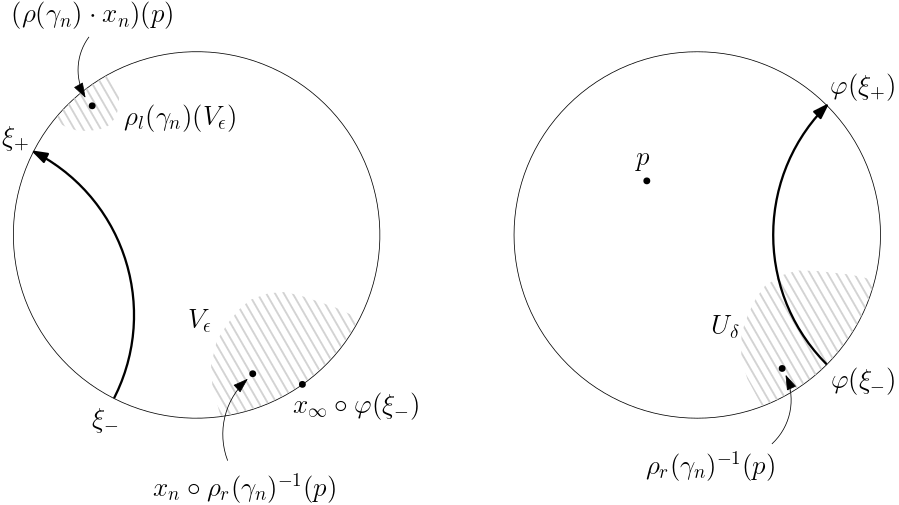
\includegraphics[width=0.7\textwidth]{dynamics.png}
%    \caption{On the proof of Prop \ref{prop:MGH_example}}
%\end{figure}
Now we prove that the MHG constructed in Proposition \ref{prop:MGH_example} are all the MGH spacetime of genus $n$.
\begin{lemma}
    Let $\rho=(\rho_l,\rho_r)$ be a pair of positive Fuchsian representations, and $\varphi :\S \to \S$ be the unique $(\rho_l,\rho_r)$-equivariant orientation-preserving homeomorphism of $\S$. Then $\Lambda(\rho)$ is the unique proper achronal meridian in $\partial \A^{2,1}$ invariant under the action of $\rho(\pi_1(\Sigma_n))$.
\end{lemma}
\begin{proof} 
    Let $\Lambda$ be a proper achronal meridian invariant under the action of $\rho(\pi_1(\Sigma_n))$. We claim $\Lambda \cap \Lambda(\rho)$ is not empty.\\
    Let $\gamma$ be a non-trivial element in $\pi_1(\Sigma_n)$. $\rho_l(\gamma)$ and $\rho_r(\gamma)$ are necessarely hyperbolic elements in $\PSL$, being $\Sigma_n$ compact, and we denote by $\xi^+_l(\gamma)$ and $\xi^+_r(\gamma)$ their attractive fixed points respectively. We have that $\xi^+_r(\gamma) = \varphi(\xi^+_l(\gamma))$, hence
    \[
        (\xi^+_l(\gamma), \xi^+_r(\gamma)) \in \Lambda(\rho).
    \]
    Now, the curve $\Lambda$ must meet the leaf of the left ruling of $\partial \A^{2,1}$
    \[
        \lambda_{\xi^+_r(\gamma)} = \{ (x, \xi^+_r(\gamma)) \ | \ x\in \S \}
    \]
    in a point $(x_0, \xi^+_r(\gamma))$. Then $(\rho_l(\gamma)^k \cdot x_0 ,\xi^+_r(\gamma)) \in \Lambda$ for $k>0$ and, if $x_0\neq \xi^-_l(\gamma)$, passing to the limit on $k$, we have that $(\xi^+_l(\gamma),\xi^+_r(\gamma))$ lies in $\Lambda$.\\
    To conclude assume by contradiction that for every $\gamma \in \pi_1(\Sigma_n)$ the point $(\xi^-_l(\gamma),\xi^+_r(\gamma))$ lies in $\Lambda$. Take $\alpha , \beta \in \pi_1(\Sigma_n)$ so that the axis of $\rho_l(\alpha)$ and $\rho_l(\beta)$ do not intersect. We may assume that the cyclic order of the end points of those axis is
    \begin{equation}\label{eq:order}
        \xi^+_l(\alpha) < \xi^+_l(\beta) < \xi^-_l(\beta) < \xi^-_l(\alpha).
    \end{equation}
    Since $\xi^\pm_r(\alpha) = \varphi(\xi^\pm_l(\alpha))$ and $\xi^\pm_r(\beta) = \varphi(\xi^\pm_l(\beta))$, Equation \ref{eq:order} holds if we replace $\rho_l$ with $\rho_r$.
    On the other hand we assumed that $\Lambda$ contains $(\xi^+_l(\alpha), \xi^-_r(\alpha))$, $(\xi^+_l(\beta), \xi^-_r(\beta))$, $(\xi^-_l(\beta), \xi^+_r(\beta))$, $(\xi^-_l(\alpha), \xi^+_r(\alpha))$. By achronality of $\Lambda$, the cyclic order of the first and second components must be the same, hence
    \[
        \xi^-_l(\alpha) \leq \xi^-_l(\beta) \leq \xi^+_l(\beta) \leq \xi^+_l(\alpha),
    \]
    which contradicts Equation \ref{eq:order}.
\end{proof}
We proved that given a pair $\rho = (\rho_l,\rho_r)$ of positive Fuchsian representations of $\pi_1(\Sigma_n)$ the MGH spacetime $M_\rho := \Omega_\rho / \rho(\pi_1(\Sigma_n))$ is the unique MGH spacetime with holonomy $\rho$.\\
The last step for the classification result is that given a MGH spacetime, the left and right components of the holonomy are necessarely positive Fuchsian.

\begin{observation}\label{rem:bundle}
    By a result of Goldman \cite{goldman1980discontinuous}, a representation $\rho$ is positive Fuchsian if and only if the associated flat $\S$ bundle $E_\rho$, constructed as the quotient of $\widetilde{\Sigma}_n \times \S$ by the diagonal action of $\pi_1(\Sigma_n)$ given by deck transformation on the first factor and by $\rho$ on the second factor, has Euler class $2-2n$. This is also equivalent to the existence of an orientation-preserving fiber bundle isomorphism between $E_\rho$ and the unit tangent bundle of $\Sigma_n$.
\end{observation}
\begin{proposition}
    Let $M$ be an oriented, time-oriented, globally hyperbolic spacetime of genus $n\geq 2$ and let us endow a Cauchy surface $\Sigma$ with the orientation induced by the future normal vector. Then the left and right components of the holonomy $\rho=(\rho_l,\rho_r): \pi_1(\Sigma)\to\PSL\times\PSL$ are positive Fuchsian representations.
\end{proposition}
\begin{proof}
    By Remark \ref{rem:bundle} we have to prove that the $\S$-flat bundles with holonomy $\rho_l$ and $\rho_r$ are isomorphic to the unit tangent bundle. We focus on $\rho_l$, the proof for $\rho_r$ is analogous.\\
    Define $\Phi_l : T^1 \widetilde{\Sigma} \to \widetilde{\Sigma} \times \S$ in the following way: for an element $(x,v) \in T^1 \widetilde{\Sigma}$ let
    \[
        \xi(x,v) = (\xi^l(x,v), \xi^r(x,v)) \in \T
    \]
    be the end-point of the spacelike geodesic ray $exp_x(tv)$ in $\A^{2,1}$, for positive $t$. We define $\Phi_l(x,v)=(x, \xi^l(x,v))$. This map is clearly continuous, proper,
    equivariant and fiber preserving.\\
    To prove that it is bijective it is sufficient to notice that for any $x \in \widetilde{\Sigma}$ the map $\xi_x : T^1_x \widetilde{\Sigma} \to \T$ is an embedding with image the boundary of the totally geodesic plane tangent to $\widetilde{\Sigma}$ at $x$. This boundary is the graph of an orientation-preserving map of $\S$, so the projection $v \to \xi^l(x,v)$ is bijective. Moreover, by the choice of the orientation on $\Sigma$, the orientation on $T^1_x \widetilde{\Sigma}$ corresponds to the orientation induced on $\xi_x (T^1_x \widetilde{\Sigma})$ as graph of an orientation-preserving homeomorphism.
\end{proof}

We conclude this section by stating the classification result. Let the \emph{deformation space} of MGH spacetimes of genus $n$ be:
$$\mathcal{MGH}(\Sigma_n)=\{g\text{ MGH AdS metric on }\Sigma_r\times\R\}/\mathrm{Diff}_0(\Sigma_n\times\R)~,$$
where the group of diffeomorphisms isotopic to the identity acts by pull-back. The holonomy map takes value in the space of representations of $\pi_1(\Sigma_r)$ into $\PSL\times\PSL$ up to conjugation and is well-defined on the quotient $\mathcal{MGH}(\Sigma_r)$.
We proved that the left and right components of the holonomy of elements of $\mathcal{MGH}(\Sigma_n)$ are positive Fuchsian representations, and the space of these representations up to conjugacy is identified with the Teichm\"uller space of $\Sigma_n$
\[
    \mathcal{T}(\Sigma_n)\cong\{\rho:\pi_1(\Sigma_n)\to\PSL\text{ positive Fuchsian representations}\}/\PSL~.
\]
Therefore the holonomy map can be considered as a map 
from $\mathcal{MGH}(\Sigma_n)$ with values in $\mathcal{T}(\Sigma_n)\times\mathcal{T}(\Sigma_n)$.
Hence, we can summarize this section with the following theorem of Mess.

\begin{theorem} \label{thm:classification rgeq2}
The holonomy map $$\rho:\mathcal{MGH}(\Sigma_n)\to\mathcal{T}(\Sigma_n)\times\mathcal{T}(\Sigma_n)$$ is a homeomorphism.
\end{theorem}

\chapter{Gauss map and spacelike immersions}

\section{Spacelike surfaces in $\A^{2,1}$}
In this section we will briefly talk about geometric properties of immersed spacelike surfaces that is analogous to the theory for the Euclidean space.\\
Let us denote with $\nabla$ the Levi-Civita connection of the Lorentzian metric of $\A^{2,1}$. Given a spacelike immersion $\sigma: S\to\A^{2,1}$ the pull-back metric $\I = \sigma^*(g_{\A^{2,1}})$ is called \textit{first fundamental form} of $\sigma$.
The tangent bundle $TS$ is naturally identified to a subbundle of the pull-back $\sigma^*(TM)$, therefore we can define its normal bundle $N_\sigma$. Using the decomposition
\[
    \sigma^* TM = TS \oplus N_\sigma \ ,
\]
the pull-back of the Levi-Civita connection $\nabla$, restricted to sections tangent to $S$ splits as the sum of the Levi-Civita connection of the first fundamental form $\I$ and a symmetric $2$-form with value in $N_\sigma$. Given the time-orientability, we take the future-directed unit normal vector field $\nu$ of $S$. The Levi-Civita connection $\nabla^\I$ of the first fundamental form $\I$ of S is defined by the relation
\begin{equation} \label{eq:levi}
    \nabla_V W= \nabla^\I_V W + \II(V,W)\nu \ ,
\end{equation} 
where the $(2,0)$-tensor $\II$ is called \textit{second fundamental form} of $\sigma$ and is defined as $\II(V,W)=\langle \nu, \nabla_V W \rangle$. The \textit{shape  operator} of $\sigma$ is the $(1,1)$-tensor $B$ defined as
\[
    B(V) = \nabla_V \nu \ .
\]
The shape operator is related to the second fundamental form by
\[
    \II(V,W) = \I(B(V),W) \ .
\]
In particular, $B$ is diagonalisable and its eigenvalues are called principal curvatures.\\

\begin{theorem}
    The first and second fundamental form of an immersion $\sigma$ satisfy the Gauss equation   
    \[
        K_\I = -1 - \text{det}B \ ,
    \]
    and the Codazzi equation
    \[
        d^{\nabla^\I}\II=0 \ ,
    \]
    where $d^{\nabla^\I}$ is the operator defined by
    \[
        (d^{\nabla^\I}\II)(X,Y,Z) = (\nabla^\I_X \II)(Y,Z) - (\nabla^\I_Y \II)(X,Z) .
    \]
\end{theorem}
\begin{proof}
    For easier computations, suppose $S \subset \A^{2,1}$. For an $X\in T\A^{2,1}$, denote by $X^\top$ and $X^\perp$ the tangent and normal part of $X$ with respect to $TS$. Using Equation \ref{eq:levi} we have
    \[
        (\nabla_X \nabla_Y Z)^\top = \nabla^I_X \nabla^I_Y Z + \II(Y,Z) \nabla_X \nu \ ,
    \] 
    \[
        (\nabla_X \nabla_Y Z)^\perp = \II(X, \nabla^I_Y Z) \nu + \partial_X (\II (Y,Z)) \nu \ ,
    \] 
    and
    \[
        (\nabla_{\left[ X,Y \right]} Z)^\top = \nabla^I_{\left[ X,Y \right]} Z \ ,
    \]
    \[
        (\nabla_{\left[ X,Y \right]} Z)^\perp = \II(\left[ X,Y \right], Z) \nu = \II(\nabla^I_X Y,Z) \nu - \II(\nabla^I_Y X,Z)\nu \ .
    \]
    Computing the tangential part of the Riemann tensor we have
    \[
    \begin{split}
        \langle R(X,Y)Z,W \rangle & = \langle R^I(X,Y)Z,W \rangle + \langle \II(Y,Z) \nabla_X \nu,  W \rangle - \langle \II(X,Z) \nabla_Y \nu, W \rangle \\
        & = \langle R^I(X,Y)Z,W \rangle - \langle \II(Y,Z) \nu, \nabla^I_X W \rangle + \langle \II(X,Z) \nu, \nabla^I_Y W \rangle \\
        & = \langle R^I(X,Y)Z,W \rangle - \II(Y,Z) \II(X,W) + \II(X,Z) \II(Y,W) \ .
    \end{split}
    \]
    Therefore the sectional curvature satisfies
    \[
        -1 = K_{\A^{2,1}} = K_I + \det(\I^{-1}\II) = K_I + \det B \ .
    \]
    Looking at the normal part of $R(X,Y)Z$ we have
    \[
    \begin{split}
        0 = \langle R(X,Y)Z,\nu \rangle & = 
        \partial_Y (\II (X,Z)) -\II(\nabla^I_Y X,Z) -\II(X, \nabla^I_Y Z) -\partial_X (\II (Y,Z)) \\ 
        & + \II(\nabla^I_X Y,Z)+\II(Y, \nabla^I_X Z) = (\nabla^I_Y \II)(X,Z) - (\nabla^I_X \II)(Y,Z).
    \end{split}
    \]
    where we used that the normal part of the Riemann tensor is null when the sectional curvature is constant (Equation \ref{sectionalcurvature}).
\end{proof}

As in the Euclidean space, the embedding data $I$ and $\II$ of a simply connected surface determines the immersion uniquely up to isometries of $\A^{2,1}$
\begin{theorem}\label{thm:immersion of simply connected surface}
    Let $S$ be a simply connected surface, let $\I$ be a Riemannian metric on $S$ and $\II$ be a symmetric $(2,0)$-tensor on $S$. If $\I$ and $\II$ satisfy the Gauss-Codazzi equations, then there exists a spacelike immersion $\sigma:S \to\A^{2,1}$ having $\I$ and $\II$ as first and second fundamental form. Moreover, if $\sigma$ and $\sigma'$ are two such immersions, then there exists a time-preserving isometry $\varphi$ of $\A^{2,1}$ such that $\sigma' = \varphi \circ \sigma$.
\end{theorem}

\section{Germs of spacelike immersions}
Let us now consider che case in which $S$ is an oriented surface, not necessarily simply connected. Let $\sigma: S \to(M,g)$ a spacelike immersion where $(M,g)$ is an oriented AdS spacetime.
As in the previous section, we can associate to $\sigma$ the pair $(\I,\II)$ of first and second  fundamental form, where $\II$ is  computed with respect to the unit future pointing normal vector $\nu$ of $\sigma$.
We will always assume that the orientation of $S$ and $\nu$ are compatible with the one on $M$.\\
We want to prove that the pair $(\I,\II)$ depends only on the \textit{germ} of $\sigma$, which is defined as follow:
\begin{definition}
    A \textit{germ} of a spacelike immersion of $S$ into an AdS spacetime is an equivalent class of spacelike immersions $\sigma:S \to(M,g)$ by the following relation: $\sigma:S \to(M,g)$ and $\sigma':S \to(M',g')$ are equivalent if there exist open subsets $U \supset \sigma(S)$ in $M$ and $U' \supset \sigma'(S)$ in $M'$ and a time-preserving isometry $f:(U,g)\to(U',g')$ such that $\sigma' = f \circ \sigma$.
\end{definition}
Given a pair $(\I,\II)$ on $S$ and $\pi: \widetilde{S}\to S$ a universal cover, one can take the pair $(\pi^*\I, \pi^*\II)$ on $\widetilde{S}$ that clearly satisfies the Gauss-Codazzi equations. By the existence part of Theorem \ref{thm:immersion of simply connected surface} there exists a spacelike immersion $\widetilde{\sigma}: \widetilde{S} \to\A^{2,1}$ having immersion data $(\pi^*\I, \pi^*\II)$.
As a coscequence of the uniqueness part of Theorem \ref{thm:immersion of simply connected surface} we have that associeted to $\widetilde{\sigma}$ there is a map $\rho:\pi_1(S) \to \text{Isom}_0(\A^{2,1})$ such that for every $\gamma \in \pi_1(S)$, $\widetilde{\sigma} \circ \gamma = \rho(\gamma) \circ \widetilde{\sigma}$.
Moreover changing $\widetilde{\sigma}$ by post-composition with an isometry $f$ of $\A^{2,1}$ has the effect of conjugating $\rho$ by $f$.
Given $\sigma:S \to \A^{2,1}$ one can extend the immersion to an immersion of an open neighbourhood of $S \times\{0\}$ in $S\times\R$ into $\A^{2,1}$, by mapping $(x,t)$ to the point $\gamma(t)$ on the timelike geodesic $\gamma$ such that $\gamma(0)=\sigma(p)$ and $\gamma'(0)$ is the future unit normal vector $\nu$ of $\sigma$ at $x$.

\begin{lemma}\label{lem:tub metric}
    Given a spacelike immersion $\sigma:S\to \A^{2,1}$, the pull-back of the ambient metric by means of the map $\sigma_t : x \to exp_{\sigma(x)}(t\nu(x))$ is given by 
    \[
        \I_t = \I((\cos(t) id + \sin(t) B)\cdot, (\cos(t) id + \sin(t) B)\cdot).
    \]
    The second fundamental form and the shape operator are given by
    \[
        \II_t = \I((-\sin(t) id + \cos(t) B)\cdot, (\cos(t) id - \sin(t) B)\cdot).
    \]
    \[
        B_t = (\cos(t) id + \sin(t) B)^{-1}(-\sin(t) id + \cos(t) B).
    \]
\end{lemma}

\begin{proof}
    By Section \ref{sec:geodesic} we have that $\sigma_t(x) = \cos(t)\sigma(x) + \sin(t) \nu(x)$.
    Then
    \[
    \begin{split}
        \I_t (v,w)& = \langle d(\sigma_t)_x (v), d(\sigma_t)_x (w) \rangle \\
        & = \langle \cos(t)d\sigma_x (v) + \sin(t)d\nu_x (v), \cos(t)d\sigma_x (w) + \sin(t)d\nu_x (w) \rangle \\
        & = \I(\cos(t) v + \sin(t) B(v), \cos(t) w + \sin(t) B(w) ).
    \end{split}
    \]
    The formula for $\II_t$ follows from the fact that $\II_t = \frac{1}{2} \frac{d \I_t}{d t}$, and the formula for $B_t$ follows from $B_t = I_t^{-1} \II_t$. 
\end{proof}


\begin{corollary}
    Given a spacelike immersion $\sigma:S\to \A^{2,1}$, the pull-back metric by means of the map $(p,t) \to exp_{\sigma(x)}(t\nu(x))$ is given by
    \begin{equation}\label{eq:tub metric}
        -dt^2 + \text{cos}^2(t)\I + 2\text{cos}(t)\text{sin}(t)\II + \text{sin}^2(t)\III,
    \end{equation}
    where $\I$, $\II$, $\III$ are the first, second and third fundamental form of $\sigma$ and third fundamental form is defined as $\III(\cdot,\cdot)=\I(B(\cdot),B(\cdot))$.
\end{corollary}
Therefore, given a pair $(\I,\II)$, Equation \ref{eq:tub metric} provides a Lorentzian metric of constant curvature $-1$ on an open neighbourhood of $S \times\{0\}$ in $S\times\R$ into $\A^{2,1}$, and thus a germ of immersion of $S$ into an AdS spacetime with immersion data $(\I,\II)$. We conclude the above discussion with the following:
\begin{proposition}\label{thm:immersion data classification}
    Given a surface $S$, there are natural identifications between the following spaces:
    \begin{itemize}
        \item The space of pairs $(\I,\II)$ on $S$ which are solutions of the Gauss-Codazzi equations,
        \item The space of germs of spacelike immersions of $S$ into Anti-de Sitter manifolds,
        \item The space of spacelike immersions of $\widetilde{S}$ into $\A^{2,1}$, equivariant with respect to a representation $\rho:\pi_1(S) \to \text{Isom}_0(\A^{2,1})$, up to the action of $\text{Isom}_0(\A^{2,1})$ by post-composition.
    \end{itemize}
\end{proposition}
%\noindent When $S$ is a closed surface the equivariant immersion $\widetilde{\sigma}$ is proper, and by Proposition \ref{prop:surface in ads} is an embedding, which can be extended to an embedding of $\widetilde{S}\times\R$ into a domain of dependence in $\A^{2,1}$. The representation $\rho:\pi_1(S) \to \PSL \times \PSL$ coincides with the holonomy of the MGH spacetime $(M,g) \cong S\times\R$, after identifying $\pi_1(S)$ with $\pi_1(M)$, and therefore $\rho$ consists of a pair $(\rho_l,\rho_r)$ of positive Fuchsian representations.\\
\noindent When $S$ is a closed surface the equivariant immersion $\widetilde{\sigma}$  by Proposition \ref{prop:surface in ads} the border at infinity of $\widetilde{\sigma}(\widetilde{S})$ is a proper achronal meridian $\Lambda$. So, $ \widetilde{\sigma}(\widetilde{S})$ is contained in the globally hyperbolic spacetime $\Omega(\Lambda)= \mathcal{\widetilde{\sigma}(\widetilde{S})}$, and therefore is contained in a maximal one.
Remarkably, the embedding data $(\I,\II)$ permits to recover an explicit pair of elements in $\mathcal{T}(S)\times\mathcal{T}(S)$ which parametrizes MGH Anti-de Sitter manifolds with compact Cauchy surfaces and in the next section we will show an explicit formula for such pair.

\section{Gauss map} \label{sec:gauss map}
We can now define the Gauss map for spacelike surfaces in $\A^{2,1}$. Recall that the space of timelike geodesics in $\A^{2,1}$ is identified with $\H^2\times\H^2$, where the identification maps a geodesic of the form
\[
    L_{p,q}=\{ X \in\PSL \ | \ X \cdot q = p \}
\]
to the pair $(p,q) \in \H^2\times\H^2$. 
\begin{definition}
    Let $\sigma :S \to\A^{2,1}$ be a spacelike immersion. The \textit{Gauss map} $G_\sigma : S \to \H^2 \times \H^2$ is defined as $G_\sigma(x) = (p,q)$ such that $L_{p,q}$ is the timelike geodesic orthogonal to $\text{Im}(d_x\sigma)$ at $\sigma(x)$.\\
    The components of the Gauss map, denoted by $\Pi_l, \Pi_r : S \to \H^2$, are called \textit{left} and \textit{right projections}. 
\end{definition}
The Gauss map $G_\sigma$ is natural with respect to the action of the isometry group, meaning that $G_{f\circ\sigma} = f \cdot G_\sigma$ for every $f \in\text{Isom}_0(\A^{2,1}) = \PSL\times\PSL$. The Gauss map is also invariant by reparametrization, in the sense that $G_{\sigma \circ \phi} = G_\sigma \circ \phi$ for a diffeomorphism $\phi:S'\to S$. Hence it makes sense to talk about the Gauss map of a spacelike surface in $\A^{2,1}$.

\begin{example}\label{ex:dual1}
    In Lemma \ref{lem:dual plane} we gave an isometric embedding of $\H^2$ in $\A^{2,1}$ with image the plane $P_{\1}$ dual to the identity. This isometric embedding was defined by sending $p\in\H^2$ to the unique order-two element in $\PSL$ fixing $p$, which by definition lies on the geodesic $L_{p,p}$. Moreover the geodesic $L_{p,p}$ is orthogonal to $P_{\1}$. Hence the Gauss map associated to this isometric embedding of $\H^2$ is just $p\mapsto (p,p).$
\end{example}
Geodesic leaving from $\1$ with velocity $\nu(p)$ meets $P_\1$ orthogonally at $\text{exp}((\pi/2)\nu(p))$, therefore, using Example \ref{ex:dual1}, one can recover the following:

\begin{lemma}\label{lem:Gaussid}
    Given a spacelike immersion $\sigma:S\to\A^{2,1}$, with future unit normal vector field $\nu$, if $\sigma(p)=\text{Id}$, then 
    \begin{equation}\label{eq:Gaussid}
        G_\sigma(p)=G_{P_\1}(\exp(\frac{\pi}{2}\nu(p))).
    \end{equation}
\end{lemma}
%\begin{proof}
%    \red{mettere proof}
    %It is a consequence of Example \ref{ex:dual1}. We need to observe that the geodesic leaving from Id with velocity $\nu(p)$ meets orthogonally $P_\text{Id}$ at $\exp((\pi/2)\nu(p)).$
%\end{proof}

Now we denote with $\hf\A^{2,1}$ the hyperboloid of future unit timelike vectors in $T_{\text{Id}}\A^{2,1}$ and consider the following map: 
\[
    \text{Fix}:T_{\text{Id}}^{1,+}\A^{2.1}\to\H^2
\]
defined so that $\text{Fix}(\nu)$ is the fixed point of the one-parameter elliptic group $\{\exp(t\nu)\;|\;t\in\R\}$. This map is equivariant for the action of $\PSL$, which acts on the hyperboloid $\hf\A^{2.1}$ by the adjoint representation and on $\H^2$ by the obvious action. Since both $\hf\A^{2.1}$ and $\H^2$ have constant curvature $-1$, it follows from equivariance that $\text{Fix}$ is an isometry.  \\
In terms of the map $\text{Fix},$ Equation \refeq{eq:Gaussid} reads as: 
\begin{equation}\label{eq:Gaussfix}
    G_\sigma(p)=(\text{Fix}(\nu(p)),\text{Fix}(\nu(p))),
\end{equation}
provided that $\sigma(p)=\text{Id}.$\\ Via Lemma \ref{lem:Gaussid} and the naturality, we can recover a different description of the Gauss map. Recalling the structure of Lie group of $\A^{2,1}\simeq\PSL$ we will denote by $R_{\gamma } $ and $L_{\gamma} $ the right and left multiplication by $\gamma\in\PSL$ respectively. 

\begin{lemma}\label{lem:gauss fix}
    Given a spacelike immersion $\sigma: S\to \A^{2.1}$ with future unit normal vector field $\nu$,
    \[
        G_\sigma(p)=(\text{Fix}((R_{\sigma(p)^{-1}})_* (\nu(p)),\text{Fix}((L_{\sigma(p)^{-1}})_* (\nu(p)))).
    \]
\end{lemma}

\begin{proof}
    If $\sigma(p)=\text{Id}$, then the equality holds true by Equation \refeq{eq:Gaussfix}. For the general case, the immersion $\sigma^{\prime} =(\text{Id},\sigma(p))\circ\sigma$ is such that $\sigma^{\prime}(p)=\text{Id}$, and the future normal vector at $\sigma^{\prime} (p)$ equals $\nu^{\prime} (p)=(R_{\sigma(p)^{-1}}))_{\ast} (\nu(p))$. Therefore: 
    \[
        G_{\sigma^{\prime} }(p)=(\text{Fix}((R_{\sigma(p)^{-1}})_{\ast} (\nu(p)),\text{Fix}((R_{\sigma(p)^{-1}})_{\ast} (\nu(p))))).
    \]
    Now by the naturality of the Gauss map it follows,     
    \begin{align*}
        G_\sigma(p)&=(\text{Id},\sigma(p)^{-1})\cdot G_{\sigma^{\prime}}(p) \\
        &=(\text{Fix}((R_{\sigma(p)^{-1}})_{\ast} (\nu(p)),\sigma(p)^{-1}\circ\text{Fix}((R_{\sigma(p)^{-1}})_{\ast} (\nu(p))))) \\
        &=(\text{Fix}((R_{\sigma(p)^{-1}})_{\ast} (\nu(p)),\text{Fix}((L_{\sigma(p)^{-1}})_{\ast} (\nu(p))))).
    \end{align*}
    where we used that Fix is equivariant with respect to the adjoint action on the hyperboloid $\hf\A^{2.1}$.
\end{proof}

%We want now to prove formulae which express the pull-back of the hyperbolic metrics by the left and right projections. When applying these formulae to the embedding data of a surface in an MGH Cauchy compact Anti-de Sitter spacetime $(M,g)$, we obtain a pair of hyperbolic metrics whose isotopy classes are the parameters of $(M,g)$ in $\mathcal{T}(S)\times\mathcal{T}(S).$
We want now to prove formulae which express the pull-back of the hyperbolic metrics by the left and right projections. When applying these formulae to the embedding data $(I,\II)$ of a closed surface $S$, we obtain a pair of hyperbolic metrics. By Proposition \ref{prop:hol} the isotopy classes of these two metric identify the parameters in $\mathcal{T}(S)\times\mathcal{T}(S)$ of a MGH spacetime $M$

\begin{observation}\label{rem:parallel transport}
    Under the identification given by Fix, the left and right projections can be interpreted in the following way. Given $p\in S$, $\Pi_l(p)$ is the parallel transport in Id of the future unit vector $\nu(p)$ at $\sigma(p)$ with respect to the right-invariant connection $D^r$. The right projection is then obtained using the left-invariant connection. 
\end{observation}

\begin{proposition}\label{prop:left right pull-back metric}
    Let $\sigma:S\to\A^{2,1}$ be a spacelike immersion, let $\Pi_l,\Pi_r:S\to\H^2$ be the left and right projections and let $g_{\H^2}$ be the hyperbolic metric. Then
    \[
        \Pi_l^*g_{\H^2}=I((\text{id}-\mathcal{J}B)\cdot,(\text{id}-\mathcal{J}B)\cdot),
    \]
        and
    \[
        \Pi_r^*(g_{\H^2})=I((\text{id}+\mathcal{J}B)\cdot,(\text{id}+\mathcal{J}B)\cdot),
    \]
    where $I$ is the first fundamental form of $\sigma$, $\mathcal{J}$ its associated almost-complex structure, and $B$ the shape operator.
\end{proposition}

\begin{proof}
    Let us check the formula for $\Pi_r$, the proof is analogous for $\Pi_l$. By Lemma \ref{lem:gauss fix}
    \[
        \Pi_r(x) = \text{Fix}((L_{\sigma(x)^{-1}})_*(\nu(x))).
    \]
    Since Fix is an isometry $\Pi^*_r g_{\H^2}$ equals the pull-back of the Anti-de Sitter metric through the map defined by $\widehat{\Pi}_r(x) = (L_{\sigma(x)^{-1}})_*(\nu(x))$.\\
    Let $X_1, X_2, X_3$ be an orthonarmal basis of left-invariant vector fields on $T\A^{2,1}$. Then the unit normal vector can be expressed as $\nu(x) = \sum_i \nu_i(x) X_i (\sigma(x))$. By Remark \ref{rem:parallel transport}
    \[
        \widehat{\Pi}_r(x) = \sum_i \nu_i(x) X_i (\1).
    \]
    Differentiating we have
    \[
        d \widehat{\Pi}_r(v) = \sum_i  d \nu_i(v) X_i (\1).
    \]
    On the other hand, since left-invariant vector fields are parallel for the left-invariant connection $D^l$, we have
    \[
        D^l_v \nu = \sum_i  d \nu_i(v) X_i (\sigma(x)).
    \]
    The last two identities show that
    \[
        \Pi_r^* g_{\H^2}(v,w) = g_{\A^{2,1}}(d \widehat{\Pi}_r(v),d \widehat{\Pi}_r(w)) = g_{\A^{2,1}} (D^l_v \nu, D^l_w \nu).
    \]
    Recalling that $\nabla_V W = D^l_V W - V \boxtimes W$ and $\left[ V,W \right] = -2 V \boxtimes W$, we have that
    \[
        D^l_v \nu = \nabla_v \nu + v \boxtimes \nu = B(v) - \nu \boxtimes v = (B- \mathcal{J})v.
    \]
    The last equality holds since $\nu$, $v$, $-Jv$ form a positive basis of $T\A^{2,1}$ and the norm of $\nu \boxtimes v$ it the product of those of $\nu$ and $v$, which together imply that $\nu \boxtimes v = -Jv$.
    We can therefore conclude that
    \[
        \Pi_r^* g_{\H^2}(v,w) = \I ((B - \mathcal{J})v, (B - \mathcal{J})w) = \I((id + \mathcal{J}B)v, (id + \mathcal{J}B)w).
    \]
\end{proof}
We collect here some consequences and remarks around Proposition \ref{prop:left right pull-back metric}.
\begin{itemize}[leftmargin=0.5cm]
\item Proposition \ref{prop:left right pull-back metric} shows that,up to post-composing with an isometry sending the image of $d_x\sigma$ to a fixed copy of $\H^2$, the differential of the left and right projections essentially has the expression 
\[
    d_x\sigma\circ(B\pm\JJ)~.
\]
Since $B$ is $\I$-symmetric $\JJ\circ B$ is traceless, and therefore 
\begin{equation}\label{eq:deteminant differential projections}
\det(B\pm\JJ)=1+\det B=-K_\I~.
\end{equation}
This shows that $\Pi_l$ is a local diffeomorphism at a point $x$ if and only if $\Pi_r$ is, which is the case if and only if the intrinsic curvature of $\I$ at $x$ is different from $0$.
\item Since the trace of $id\pm\JJ B$ equals $2$, the differentials of $\Pi_l$ and $\Pi_r$ have either rank 2 or rank 1. (In fact, by Equation \eqref{eq:deteminant differential projections}, when the differential of $\Pi_l$ has rank 1, the same holds for the differential of $\Pi_r$.) Hence the differential of the Gauss map $G:S\to\H^2\times\H^2$ is always non-singular.
\item If an immersed surface has the property that the curvature of the first fundamental form never vanishes, and if $\Pi_l$ and $\Pi_r$ are globally injective, then the image of $G$ is the graph of a  diffeomorphism $F_\sigma$ between two subsets of $\H^2$,  called the \emph{associated map}. From Equation \eqref{eq:deteminant differential projections}, the Jacobians of $\Pi_l$ and $\Pi_r$ are equal, hence the associated map is area-preserving.
When $\Pi_l$ and $\Pi_r$ are only locally injective, but not globally, we still obtain an area-preserving local diffeomorphism $F_\sigma$ which is now defined between two hyperbolic surfaces.
\item More generally, as a consequence of the previous points, the image of $G$ is always a \emph{Lagrangian submanifold} in $\H^2\times\H^2$ with respect to the symplectic form 
\begin{equation} \label{eq symplectic form}
\Omega=\pi_l^*\omega_{\H^2}-\pi_r^*\omega_{\H^2}~,
\end{equation}
where $\omega_{\H^2}$ is the hyperbolic area form. 
This result has been proved in several works with different methods: see \cite{bonsante2017equivariant}, \cite{Seppi_2017}. Moreover the Lagrangian condition is \emph{locally} the only obstruction to inverting this construction, that is, to realizing an immersed surfaces in $\H^2\times\H^2$ locally as the image of the Gauss map of a spacelike immersion in $\A^{2,1}$.
\item Given a spacelike immersion $\sigma$,  the normal evolution of $\sigma$ is defined as 
\[
    \sigma_t(x)=\exp_{\sigma(x)}(t\nu(x))~,
\]
where $\nu$ is the future unit normal vector field. When it is an immersion, the computation of the metric in Lemma \ref{lem:tub metric} shows that the image of $\sigma_t$ at $x$ is orthogonal to the geodesic $\gamma(t)=\exp_{\sigma(x)}(t\nu(x))$. In other words, the Gauss map of $\sigma_t$ is equal to the Gauss map of $\sigma$. 
\end{itemize}

We conclude this section with the following:

\begin{proposition} \label{prop:Gaussian curvature}
    Let $S$ be a surface with a Riemannian metric $\I$. Let $A$ be a $(1,1)$-tensor which is $\I$-symmetric and $\I$-Codazzi, which means that $d^{\nabla^{\I}} A=0$. Then the curvature of $g= \I(A \cdot, A \cdot)$ is given by
    \[
        K_g = \frac{K_\I}{det(A)}.
    \]
\end{proposition}
\begin{proof}
    First we prove that the Levi-Civita connection of the metric $g$ is given by
    \[
        \nabla^g_X Y = A^{-1} \nabla^I_X(AY) \ .
    \]
    It is torsion-free, for all $X,Y$
    \[
    \begin{split}
        \nabla^g_X Y - \nabla^g_Y X & =  A^{-1} \nabla^I_X(AY) - A^{-1} \nabla^I_Y(AX) \\
        & = A^{-1} (\nabla^I_XA)Y + \nabla^I_X Y - A^{-1} (\nabla^I_YA)X - \nabla^I_Y X  \\
        & = A^{-1} d^{\nabla^I}A(X,Y) +  \nabla^I_X Y - \nabla^I_Y X = 0 \ ,
    \end{split}
    \]
    since $\nabla^I$ is torsion-free and $d^{\nabla^I}A = 0$. $\nabla^g$ is also compatible with $g$ since for all $X,Y,Z$
    \[
    \begin{split}
        \partial_Z g(X,Y) & = \partial_Z I(AX,AY) \\
        & = I(\nabla^I_Z(AX),AY) + I(AX,\nabla^I_Z(AY)) \\
        & = g(A^{-1}\nabla^I_Z(AX),Y) + g(X,A^{-1}\nabla^I_Z(AY)) \\
        & = g(\nabla^g_Z X,Y) + g(X, \nabla^g_Z Y) \ .
    \end{split}
    \]
    Let now $(e_1, e_2)$ be an orthonormal frame on $S$ for the metric $\I$. It is known that for an orthonormal frame on a surface
    \[
        \nabla^I_X e_1 = \beta(X)e_2 \ , \qquad \nabla^I_X e_2 = -\beta(X)e_1 \ ,
    \]
    where $\beta$ is the connection $1$-form for the metric $\I$, and the curvature $K_I$ can be defined as $d\beta = -K_I \omega_I$, where $\omega_I$ is the volume form on $S$. Let now $(e_1', e_2') = (A^{-1} e_1, A^{-1} e_2)$ be the orthonormal frame for $g$, then
    \[
        \nabla^g_X e_1' = A^{-1} \nabla^I_X Ae_1' = \beta(X) A^{-1} e_2 = \beta(X) e_2' \ ,
    \]
    which shows that $\beta$ is also the connection form for $g$. It follows that 
    \[
        d\beta = - K_g \omega_g = - K_I \omega_I \ ,
    \]
    and therefore
    \[
        K_g = K_I \frac{\omega_I}{\omega_g} = \frac{K_I}{det A} \ .
    \]
\end{proof}
Applying the proposition to the tensors $id \pm \mathcal{J} \circ B$, Equation (\ref{eq:deteminant differential projections}) shows that the pull-back metrics defined in Proposition \ref{prop:left right pull-back metric}, when non-degenerate, are always hyperbolic.

\chapter{Minimal Lagrangian diffeomorphism}

\red{Minimal surfaces and particles in 3-manifolds lemma 3.3: ad ogni superficie massimale si può associare un unico GHM spacetime}


\red{aggiungere intro?}
\section{CMC Surfaces}
A smoothly embedded spacelike surface $S$ has \textit{constant mean curvature} if the trace of the shape operator $B$ is constant. A \textit{maximal surface} is a surface $S$ whose mean curvature is constantly equal to zero.
\begin{theorem}\label{thm:CMC_foliation}
    Every MGH Anti-de Sitter manifold with compact Cauchy surface is uniquely foliated by closed CMC surfaces, where the mean curvature $H$ varies in $(-\infty,\infty)$. In particular every MGH Anti-de Sitter manifold with compact Cauchy surface admits a unique maximal surface.
\end{theorem}
The proof of theorem \ref{thm:CMC_foliation} can be found in \cite{barbot2004constant} and revolves around the existance of a pair of barriers, which are two surfaces with everywhere positive/negatime mean curvature, respectively.\\
Using the normal evolution
\[
    \sigma_t(x) = \text{exp}_{\sigma(x)} (t\nu(x))
\]
one can find a relation between CMC and CGC surfaces:
\begin{proposition}
    Let $\sigma: S \to\A^{2,1}$ be an immersion of constant Gaussian curvature $K>0$. Then the normal evolution $\sigma_{t_K}$ on the convex side of $\sigma$, for time $t_K=\text{arctan}(K^{1/2})$, is an immersion of constant mean curvature $H=K^{-1/2}(K-1)$.
\end{proposition}
\begin{proof}
    By Lemma \ref{lem:tub metric} the first fundamental form $\I_t$ of $\sigma_t$ is given by
    \[
        \I_t(\cdot, \cdot) = \I((\cos(t)id + \sin(t)B)\cdot, (\cos(t)id + \sin(t)B)\cdot).
    \]
    Let us denote by $B_t$ the shape operato of $\I_t$. By Remark \ref{prop:Gaussian curvature} we have
    \[
        K_I = \frac{K_{\I_t}}{det(\cos(t)id - \sin(t)B_t)} = - \frac{1+detB_t}{det(\cos^2(t) + \sin^2(t)det B_t -\cos(t) \sin(t)tr B_t)}.
    \]
    Hence $K_I$ is constant if and only if $tr B_t = 2/ \tan(2t)$, that happens for $\tan(t) = 1 / \sqrt{K}$.
\end{proof}

\section{Minimal Lagrangian diffeomorphism}

\red{da finire}
\begin{definition}
    Let $h$ and $h'$ be two hyperbolic metrics on the closed surface $S$. A diffeomorphism $f: (S,h) \to (S,h')$ is \textit{minimal Lagrangian} if its graph is a minimal Lagrangian submanifold of $S\times S$ with respect to the product metric $h \oplus h'$ and the symplectic form $\pi_l^*\omega_h - \pi_r^* \omega_{h'}$. 
\end{definition}

\red{la convessità di alcune cose ci dà che B è def positivo e quindi che le proiezioni sono diffeo loc (se non sbaglio)}
%Sep17,  BS10

%\include{conclusione}
%\appendix
%\include{appendice}
\printbibliography
\end{document}
